% The sections on linear regression and linear mixed models are similar to those presented in the authors project thesis \citep{Arnstad:Relative_variable_importance_in_Bayesian_linear_mixed_models:2024}, which lead up to the masters thesis.
\section{Linear regression}
\label{sec:linreg}
All regression models are based on the assumption that the response variable is influenced by one or more covariates (regressors).
The relationship between the response and the covariate is assumed not to be deterministic, so we expect our modelling of the response to be influenced by some random error \citep{GLMM_book}.
This means that the response is treated as a random variable, and it is desirable to decompose the response into systematic components and random components. Throughout this section, we will mostly follow the derivations of \citet{GLMM_book} and \citet{GLMM_book_old}.
\subsection{Linear regression}
Assuming that an observed response $y_i$ has a linear relationship with a covariate $x_i$ is the basis for the simple linear regression.
This can be modeled by the equation
\begin{equation}
    y_i = \beta_0 + \beta_1x_i + \varepsilon_i \ ,
\end{equation}
where $\beta_0$ is the intercept, $\beta_1$ is the slope, and $\varepsilon_i$ is the error term.
The error term, or residual, is assumed to be normally distributed with mean zero and variance $\sigma^2$, i.e. $\varepsilon_i \sim \mathcal{N}(0, \sigma^2)$.
Generalizing to multiple covariates is straightforward by defining the $n\times p$ matrix $\mathbf{X}$ as a design matrix with, including an intercept, the $p$ covariates in the columns and the $n$ observations in the rows.
With this definition, the linear regression model can be written as
\begin{equation}
    \label{eq:linreg}
    \mathbf{y} = \mathbf{X}\boldsymbol{\beta} + \mathbf{\varepsilon} \ ,
\end{equation}
where now $\mathbf{y}=(y_1, y_2, ..., y_n)$ is a vector of $n$ responses, $\boldsymbol{\beta}=(\beta_0, \beta_1, ..., \beta_{p-1})$ is a vector of coefficients including the intercept $\beta_0$, and $\mathbf{\varepsilon}=(\varepsilon_1, \varepsilon_2, ..., \varepsilon_n)$ is a vector of error terms.
The error terms are assumed to be independent and identically distributed (i.i.d.) with $\boldsymbol{\varepsilon} \sim \mathcal{N}(0, \sigma^2 \mathbf{I})$, where $\mathbf{I}$ is the identity matrix of size $n \times n$.
Consequently, the response $\mathbf{y}$ is conditionally independent given the covariates $\mathbf{X}$, i.e.
\begin{equation}
    \mathbf{y} \lvert \mathbf{X} \sim \mathcal{N}_n(\mathbf{X}\boldsymbol{\beta}, \sigma^2\mathbf{I}) \ .
\end{equation}
In practice, the coefficients $\boldsymbol{\beta}$ are estimated from the maximum likelihood estimation (MLE) method, given by
\begin{equation}
    \label{eq:beta_hat}
    \hat{\boldsymbol{\beta}} = (\mathbf{X}^T\mathbf{X})^{-1}\mathbf{X}^T\mathbf{y} \ .
\end{equation}

\subsection{Qualitative covariates}
\label{sec:qualitative}
In many cases the covariates are qualitative, meaning they are categorical variables that can be grouped into different levels or factors.
Qualitative covariates, unlike quantitative, cannot be measured numerically, and we must adjust our modelling to account for this.
A common approach to model qualitative data is to include dummy variables, which are assigned a value $1$ if the observation is in the respective category(factor) and $0$ otherwise.
Given $N$ factors, it is standard practice to model $N-1$ dummy variables and let one factor be captured by the intercept to uniquely determine the model.
Dummy encoding in this way retains the properties of the linear regression, and is limited by the same assumptions.
The model for the response $y_i$, assuming no quantitative covariates, from group $j$ with dummy encoding is then given by
\begin{equation}
    y_i =  \beta_0 + \sum_{j=1}^{N-1} \beta_j x_{i,j} + \varepsilon_i \ ,
\end{equation}
where $\beta_j$ denotes the factor coefficient of observation $i$ and the dummy variable
\begin{equation}
    x_{i,j} = \begin{cases}
        1 & \text{if observation $i$ is in group $j$} \\
        0 & \text{otherwise}
    \end{cases} \ .
\end{equation}
This way of modelling qualitative covariates is intuitive and easy to interpret, but it also assumes that factor specific effects are uniform and fixed across all levels and becomes cumbersome with many categorical covariates. 

\subsection{Correlation among covariates in linear regression}
Correlation among covariates is to be expected, as it is natural in many practical applications. However, if the correlation is very strong, this poses some serious problems when interpreting the linear regression model.
The covariates $\mathbf{x}_i$ in a linear regression are assumed to be linearly independent, so that the design matrix $\mathbf{X}$ has full rank.
If the design matrix is not of full rank, that is one or more covariates are perfectly correlated, the model \eqref{eq:linreg} is said to be \textit{multicollinear} \citep{Poole_OFarrell_1971}. 
From \eqref{eq:beta_hat} one can see that if the matrix $\mathbf{X}$ is not of full rank, the term $(\mathbf{X}^T\mathbf{X})^{-1}$ is not invertible and the MLE of $\boldsymbol{\beta}$ does not exist. 
Further, the variance of the MLE of $\boldsymbol{\beta}$ grows as the correlation between covariates grows \citep[p. 116]{GLMM_book}. A larger variance in $\boldsymbol{\hat{\beta}}$ also leads to larger standard errors for $\boldsymbol{\hat{\beta}}$, making it hard to assess the model.
Both coefficients and covariates affect the total marginal model variance, which can be decomposed as
\begin{equation}
    \label{eq:var_y}
    \text{Var}(\mathbf{y}) = \text{Var}(\mathbf{X}\boldsymbol{\beta}) + \text{Var}(\boldsymbol{\varepsilon}) = \boldsymbol{\beta}^T\mathbf{V}\boldsymbol{\beta} + \sigma^2_{\varepsilon} = \sum_{j=1}^p\beta_j^2v_j +\sum_{j=1}^{p-1}\sum_{k=j+1}^{p} \beta_j\beta_k\sqrt{v_jv_k}\rho_{jk} + \sigma_{\varepsilon}^2 \ ,
\end{equation}
where $\mathbf{V} = \text{Cov}(\mathbf{X})$ is the $p \times p$ covariance matrix of the covariates which is assumed to be positive definite, $\boldsymbol{\beta}$ is the $p \times 1$ vector of regression coefficients, $v_j$ the regressor variances for $j=1, ..., p$ found along the diagonal of $\mathbf{V}$ and $\rho_{jk}$ the inter-regressor correlations between regressor $j$ and $k$ \citep{gromping_relaimpo}.
The middle term in \eqref{eq:var_y} consist of the covariance between the covariates and the variance contribution from a single covariate is not immediately clear.

%this term makes it hard to assess the relative importance of each covariate. 
%To assign each covariate with an importance, we need to consider relative importance measures that can handle the correlation among covariates.

%\subsection{Relative variable importance \protect\footnote{This subsection is slightly modified from the project thesis \citep{Arnstad:Relative_variable_importance_in_Bayesian_linear_mixed_models:2024}.}} 
\section{Variable importance in linear regression models}
In a regression setting with multiple regression coefficients, it is often desirable to be able to assign each covariate with a measure of its relative importance with respect to the model.
The relative importance of covariate $\mathbf{x}_i$ is defined as the standardized contribution to explained variance in the response $\mathbf{y}$ from $\mathbf{x}_i$ \citep{gromping_relaimpo}.
Assigning relative importance is no trivial task, as correlation among covariates poses a challenge in assessing the relative importance of each covariate.
\newline
\newline



\subsection{Relative importance measures}
\label{sec:rel_imp}
The coefficient of determination, $R^2$, is a widely used and intuitive summary statistic of goodness-of-fit, which can also be used for model comparison. 
Conceptually, the $R^2 \in [0, 1]$ and quantifies the proportion of variance in the response variable that can be attributed to the covariates in the model. 
For the linear regression model, the $R^2$ is defined as
\begin{equation}
    \label{eq:R2}
    R^2 = 1 - \frac{(\mathbf{y}-\mathbf{X}\boldsymbol{\beta})^T(\mathbf{y}-\mathbf{X}\boldsymbol{\beta})}{(\mathbf{y}-\overline{\mathbf{y}})^T(\mathbf{y}-\overline{\mathbf{y}})} = \frac{\text{Var}(\mathbf{y}) - \sigma^2_{\varepsilon}}{\text{Var}(\mathbf{y})} \ ,
\end{equation}
where $\overline{\mathbf{y}}$ is the mean vector of responses $\mathbf{y}$. 
Instead of referring to the $R^2$ value alone, going forward this thesis will focus on decomposing of the $R^2$ value and allocate a proportion of $R^2$ to the model covariates. 
This decomposition is done in order to assess the relative importance, or variance explained, of each covariate in the model.
% Generally, the variance of a linear regression model can be stated as in equation \eqref{eq:var_y}, however in the case of 
The special case of uncorrelated covariates in \eqref{eq:var_y} gives 
% we obtain  
\begin{equation}
    \label{eq:var_y_uncorrelated}
    \text{Var}(\mathbf{y}) = \sum_{j=1}^p\beta_j^2v_j + \sigma_{\varepsilon}^2 \ ,
\end{equation}
% This case
% , the $R^2$ is consistent with the proportion of variance explained in the response total variance of the response variable \citep{gromping_relaimpo}. 
% This consistency 
and provides a natural decomposition of the $R^2$ in terms of contribution from each covariate, as each predictor $\mathbf{x}_i$ contributes $\beta_i^2v_i$ to the total response variance \citep{gromping_relaimpo}.
In \eqref{eq:var_y} however, the response variance is split into three parts, the first two sums which comes from the regressors and the latter term which is the variance of the error. 
As mentioned, it is the middle term that poses the problem of assigning importance to each covariate, since it is not immediately clear how to distribute the total response variance to each covariate, as some variance contributions in the response variance are shared among covariates. The literature has established some criteria that relative importance measures should fulfill, so that they can be interpreted and compared in a sensible manner \citep{gromping_relaimpo}. As listed in \citet{gromping_relaimpo}, the methods should yield
\begin{enumerate}
    \label{list:criteria}
    \item \textbf{Proper decomposition}: The model variance should be decomposed into shares for each regressor that sum up to the total variance, and the method shall allocate the shares to each regressor.
    \item \textbf{Non-negativity}: Each share of the variance should be non-negative.
    \item \textbf{Exclusion}: If a regressor is excluded from the model, $\beta_j=0$, its share of the variance should be zero.
    \item \textbf{Inclusion}: If a regressor is included in the model, $\beta_j \neq 0$, its share of the variance should be positive.
\end{enumerate}
Further, \citet{gromping_relaimpo} introduces some useful notation for considering variable importance, for the explained variance of a subset of regressors $S$ as 
\begin{equation}
    \text{evar}(S) = \text{Var}(\mathbf{y}) - \text{Var}(\mathbf{y} \lvert \mathbf{x}_j, j\in S) \ ,
\end{equation}
and the added explained variance of a subset $M$ to a model that already contains the covariates in $S$ as
\begin{equation}
    \text{svar}(M \lvert S) = \text{evar}(M \cup S) - \text{evar}(S) \ .
\end{equation}

% \begin{equation}
%     \label{eq:var_y_full}
%     \text{Var}(\mathbf{y}) = \sum_{j=1}^p\beta_j^2v_j + \sum_{j=1}^{p-1}\sum_{k=j+1}^{p} \beta_j\beta_k\sqrt{v_jv_k}\rho_{jk} + \sigma_{\varepsilon}^2 \ ,
% \end{equation}
% where $\beta_j$ is the $j$-th regression coefficient, $v_j$ is the variance of the $j$-th covariate, $\rho_{jk}$ is the correlation between the $j$-th and $k$-th covariate and $\sigma_{\varepsilon}^2$ is the variance of the error term.
\subsection{Naive decompositions of \texorpdfstring{$R^2$}{Lg}}
\label{sec:naive_decomp}
To make it clear that some simple decompositions fail the criteria of relative importance measures, we will consider two naive approaches for decomposing the $R^2$. We denote the $R^2$ of a linear regression with regressors $X_1, \dots, X_p$ as $R^2(\{1, \dots, p\})$ and the relative importance of regressor $X_i$ as $\text{RI}(\{i\})$.
\newline
\newline
The first naive method is to fit a model with all regressors $p$, and then fit a model with all regressors excluding regressor $i$. The relative importance of $X_i$ is then the difference $R^2(\{1, \dots, p\}) - R^2(\{1, \dots, p\} \setminus i)$.
To show how this fails the criteria of relative importance measures, an example from \citet{matre} is discussed. The example considers the simple case 
\begin{equation}
    Y=X_1+X_2, \quad \text{Var}(X_1) = \text{Var}(X_2)=1, \quad \text{Cov}(X_1, X_2)=0.9 \ .
\end{equation}
The $R^2$ of the model with both covariates is $R^2(\{1, 2\})=1$, since the covariates $X_1, X_2$ explain fully the response $Y$. Then one would expect that the importance of $X_1$ and $X_2$ is $0.5$ each, since they both explain half of the response variance.
Using the proposed decomposition, one would calculate
\begin{equation}
    \text{RI}(\{2\}) = R^2(\{1, 2\}) - R^2(\{1\}) = 1 - \frac{\text{Cov}(Y, X_1)^2}{\text{Var}(Y)\text{Var}(X_1)} = 1- \frac{1.9^2}{3.8} \approx 0.05 \ ,
\end{equation}
where it is used that for the simple linear regression, the $R^2$ is given by the squared correlation coefficient between the response and the regressor.
By symmetry $\text{RI}(\{1\})=\text{RI}(\{2\})$, so the sum of the relative importances is $0.1$. However, the total explained variance of the model is $1$, so this decomposition violates the proper decomposition condition.
This decomposition only assign importances to the regressor based on the information that the regressor does not share with any other regressors. Therefore, it does not take into account the shared information and the importance estimated is too low.
\newline
\newline
Another naive decomposition would be to compare the relative importance of a model with one regressor $i$ to the empty model, \textit{i.e.} the model with no covariates. 
The empty model has an $R^2=0$ and therefore for $X_1$ in the above example we would have
\begin{equation}
    \text{RI}(\{1\}) = R^2(\{1\}) - R^2(\{\emptyset\}) = \frac{\text{Cov}(Y, X_1)^2}{\text{Var}(Y)\text{Var}(X_1)} = \frac{1.9^2}{3.8} \approx 0.95 \ .
\end{equation}
Once more by symmetry we have $\text{RI}(\{2\})=\text{RI}(\{1\})$, so the sum of the relative importances is $1.9$, violating the proper decomposition condition.
In contrast to the first naive approach, this decomposition assigns importances based on the full information contained in the regressor. Therefore, it overestimates the importance of each variable, since the shared information is accounted for twice.
\newline
\newline
As we have seen from these naive approaches, the task of decomposing the $R^2$ value is far from trivial, and calls for more sophisticated methods.

\subsection{The Lindemann, Merenda and Gold(LMG) method}
\label{sec:lmg}
A method that handles correlation among covariates, and is frequently reinvented from different approaches, is the Lindemann, Merenda and Gold (LMG) method \citep{gromping_relaimpo}.
We shall therefore discuss it, as it serves an important role as a leading method for assigning relative variable importance.  
The LMG method takes use of averaging over orders, meaning that it permutes the index set $\{1, ..., p\}$  of the regressors $(p-1)!$ times, excluding the intercept, and sequentially adds the regressors to the model for each permuted index set.
By adding regressors sequentially for each permutation, one can investigate how the importance of the regressors vary depending on what other regressors are included, which is useful when they are correlated.
This is justified by the assumption that there is no relevant ordering of the regressors in the index set \citep{kruskal_lmg_1987}.
For each regressor added, starting with none, it allocates a share of explained variance, or importance, and then adds a new regressor.
The final allocated share to the regressor is the average of the allocated shares to that regressor for all permutations of the set of regressors indices. 
This would mean that for two correlated regressors whose importance share varies depending on which is added first, would receive an averaged importance.
Averaging over orders is a statistical tradition \citep{kruskal_lmg_1987} and gives a robust assessment of each regressor's importance by considering different orderings of how they are added to the model. 
The iterative process for the regressors $\{X_0, X_1, X_2, X_3\}$, where $X_0$ is the intercept, would be
\begin{enumerate}
    \item Considering $\{X_1, X_2, X_3\}$,  $X_1$ is added to the model, and the share of explained variance allocated to $X_1$ is $\text{svar}(\{1\} \lvert \emptyset)$. $X_2$ is added and allocated a share of $\text{svar}(\{2\} \lvert \{1\})$, and lastly $X_3$ is added and allocated a share of $\text{svar}(\{3\} \lvert \{1, 2\})$.
    \item Considering $\{X_1, X_3, X_2\}$,  $X_1$ is added to the model, and the share of explained variance allocated to $X_1$ is $\text{svar}(\{1\} \lvert \emptyset)$. $X_3$ is added and allocated a share of $\text{svar}(\{3\} \lvert \{1\})$, and lastly $X_2$ is added and allocated a share of $\text{svar}(\{2\} \lvert \{1, 3\})$.
\end{enumerate}
The above iteration is repeated for all 6 possible permutations of orderings among regressors to obtain the final result.
This iterative process gives rise to the general formula for share of explained variance allocated to $X_1$ by the LMG method with $p$ regressors,
\begin{equation}
    \label{eq:LMG}
    \text{LMG}(1) = \frac{1}{p!} \sum_{S \subseteq \{2, ..., p\}} n(S)! (p - n(S)-1)! \text{svar}(\{1\} \lvert S) \ ,
\end{equation} 
where $n(S)$ is the number of regressors in $S$ \citep{gromping_relaimpo}.
Equation \eqref{eq:LMG} averages the increase in $R^2$, $\text{svar}(\{X_i\})$, when adding the covariate of interest, $X_i$, over all possible orderings of covariates. 
This mean increase over orderings is assigned as the proportion of $R^2$ explained by $X_i$.
The LMG method fulfills all but the exclusion criteria described previously \citep{gromping_relaimpo}, but \citet{gromping_relaimpo} argues that this \textit{"must be seen as a natural result of model uncertainty"} and therefore that this criterion is not indispensable.
Therefore, we find it also suitable for our purposes to focus on the three other criteria.
The setback of the LMG method is the great computational expense that the permutations require when $p$ is large. The complexity is $2^{p-1}$ summations \citep{gromping_relaimpo}, and therefore, the LMG is not suitable for high dimensional models. 



\subsection{Relative weights method}
\label{sec:relativeweights}
A method that takes advantage of the straightforward decomposition of the variance when the fixed covariates are uncorrelated is the relative weights method \citep{johnson_relative_weights}, which will now be discussed.
\newline
\newline
The relative weights method proposes an alternative to the LMG, which is significantly less computationally expensive. 
Intuitively, the relative weights method projects the design matrix $\mathbf{X}$ of the fixed effects into an orthogonal column space, resulting in a matrix $\mathbf{Z}$ with orthogonal columns.
The matrix $\mathbf{Z}$ is then an approximation of $\mathbf{X}$ and will be used as the design matrix in the regression. Since the columns of the design matrix $\mathbf{Z}$ are orthogonal, each covariate is uncorrelated. 
This allows us to decompose the variance in the straightforward manner as in equation \eqref{eq:var_y_uncorrelated}.
% As is mentioned above, decomposing the variance with uncorrelated predictors is straightforward. To see this, one can with out loss of generalization, standardize the repsonse to have the zero-vector as mean and the identity matrix as variance. Then it is clear that the marginal variance can be found as
% \begin{equation}
%     \text{Var}(\mathbf{y}) = \text{Var}(\mathbf{X}^T\boldsymbol{\beta} + \boldsymbol{\varepsilon}) = \boldsymbol{\beta}^T\text{Var}(X)\boldsymbol{\beta} + \sigma^2 = \boldsymbol{\beta}^T\boldsymbol{\beta} + \sigma^2 \ ,
% \end{equation}
% so for each predictor the contribution to the full explained variance is the corresponding regression coefficient squared. This property lies the foundation for the relative weights method, which will now be considered.
\newline
\newline
In relative weights one uses the singular value decomposition \citep{relative_weights_nimon_oswald}, to project the real-valued design matrix $\mathbf{X}$ into an orthonormal matrix $\mathbf{U} \in \mathbb{R}^{n \times n}$ containing the eigenvectors of $\mathbf{X}\mathbf{X}^T$, an $n\times p$ diagonal matrix $\mathbf{D}$ containing the singular values of $\mathbf{X}$ and another orthonormal matrix $\mathbf{V} \in \mathbb{R}^{p \times p}$ containing the eigenvectors of $\mathbf{X}^T\mathbf{X}$ such that
%The above matrix relations differ from Matre, double check them!
\begin{equation}
    \label{eq:SVD}
    \mathbf{X} = \mathbf{UDV^T} \ .
\end{equation}
From the Eckhart-Young-Mirsky theorem \citep{mirsky-theorem} and following the derivations of \citet{johnson_minimization_trace}, one can state that the matrix $\mathbf{X}$, of rank $r$, can be approximated by a matrix $\mathbf{Z} = \mathbf{U}\mathbf{V}^T$ of rank $k\leq r$ such that the difference under the squared Frobenius norm
\begin{equation}
    \lVert \mathbf{X} - \mathbf{Z} \rVert_F^2 = tr \left( (\mathbf{X} - \mathbf{Z})^T(\mathbf{X} - \mathbf{Z}) \right) \ ,
\end{equation}
is minimized. The relative weights approximation now utilizes the matrix \citep{johnson_relative_weights} $\frac{1}{\sqrt{n-1}}\mathbf{{Z}}$, where the factor $\frac{1}{\sqrt{n-1}}$ is the standardization factor for $\mathbf{Z}$ \citep{matre}, and regresses on $\mathbf{Z}$ to find the MLE $\boldsymbol{\beta_Z}$ as
\begin{equation}
    \begin{aligned}
        \boldsymbol{\beta_Z} & = (\mathbf{Z}^T\mathbf{Z})^{-1}\mathbf{Z}\mathbf{y} \\
        & = \left((n-1) \mathbf{VU}^T\mathbf{UV}^T \right)^{-1} \sqrt{n-1}\mathbf{VU}^T\mathbf{y} \\
        & = \frac{1}{\sqrt{n-1}}\mathbf{V}\mathbf{U}^T\mathbf{y} \ .
    \end{aligned}
\end{equation} 
As $\mathbf{Z}$ is orthogonal, the relative importance for each column $\mathbf{z_i}$ with respect to the response $\mathbf{y}$ can be found as the square of $\beta_{Z, i}^2$, denoted as $\boldsymbol{\beta_Z}^{[2]}$. 
The notation $\boldsymbol{\xi}^{[2]}$ for some $\boldsymbol{\xi}$ represents the Schur product of $\boldsymbol{\xi}$ with itself, \textit{i.e.} element wise squaring of each element in $\boldsymbol{\xi}$.
Once these importances are obtained, \citet{johnson_relative_weights} argues that we should regress $\mathbf{X}$ on $\mathbf{Z}$ to obtain the weights that relate the importance of each column of $\mathbf{Z}$ to each column of $\mathbf{X}$. These weights can be calculated as the matrix
\begin{equation}
    \label{eq:lambda_rw}
    \boldsymbol{\Lambda} = (\mathbf{Z}^T\mathbf{Z})^{-1}\mathbf{Z}^T\mathbf{X} = (\mathbf{V}\mathbf{U}^T\mathbf{U}\mathbf{V}^T)^{-1}\mathbf{V}\mathbf{U}^T\mathbf{U}\mathbf{D}\mathbf{V}^T = \mathbf{V}\mathbf{D}\mathbf{V}^T \ ,
\end{equation}
and since $\mathbf{Z}$ is orthogonal, the contribution from a column of $\mathbf{z_i}$ with respect to a column $\mathbf{x}_j$ is the squared entry $\boldsymbol{\Lambda}_{ij}^2$.
The contribution from a column $\mathbf{x}_j$ with respect to the response $\mathbf{y}$, \textit{i.e.} the relative importance, is then estimated as the matrix product \citep{johnson_relative_weights}
\begin{equation}
    \label{eq:RI_lambda}
    \text{RI}(\mathbf{X}) = \boldsymbol{\Lambda}^{[2]} \boldsymbol{\beta_Z}^{[2]} \ , 
\end{equation}
with $\text{RI}$ as a column vector where each entry $j$ contains the estimate of the relative importance corresponding to column $j$ of $\mathbf{X}$.
In \citet[section 2.5.3]{matre} it is shown that the relative weights method fulfills the criteria same three criteria as the LMG method, because $\mathbf{Z}$ and $\mathbf{X}$ are linear combinations of each other and due to the properties of $\boldsymbol{\Lambda}$.



% \newline
% \newline
% Due to the popularity of $R^2$, it is desirable to also be able to decompose the $R^2$ in the case of correlated covariates, such that it is consistent with the variance of the response.
% In (\ref{eq:var_y_full}) the response variance is split into three parts, the first two sums which comes from the regressors and the latter term which is the variance of the error. 
% It is the middle term that poses the problem of assigning importance to each covariate, since it contains the covariance between the covariates.
% The literature has established some conditions that relative importance measures should fulfill, so that they can be interpreted and compared in a sensible manner \citep{gromping_relaimpo}. As listed in \citet{gromping_relaimpo}, the methods should have
% \begin{enumerate}
%     \label{list:criteria}
%     \item \textbf{Proper decomposition}: The model variance should be decomposed into shares for each regressor that sum up to the total variance, and the method shall allocate the shares to each regressor.
%     \item \textbf{Non-negativity}: Each share of the variance should be non-negative.
%     \item \textbf{Exclusion}: If a regressor is excluded from the model, $\beta_j=0$, its share of the variance should be zero.
%     \item \textbf{Inclusion}: If a regressor is included in the model, $\beta_j \neq 0$, its share of the variance should be positive.
% \end{enumerate}
% Before moving on the such methods, some notation in accordance with \citet{gromping_relaimpo} will be introduced, namely
% \begin{equation}
%     \text{evar}(S) = \text{Var}(Y) - \text{Var}(Y \lvert X_j, j\in S) 
% \end{equation} 
% and
% \begin{equation}
%     \text{svar}(M \lvert S) = \text{evar}(M \cup S) - \text{evar}(S) \ ,
% \end{equation} 
% where $S$ is a subset of regressors, $\text{Var}(Y \lvert X_j, j\in S)$ denotes the variance of $Y$ conditioned on $X_j, j\in S$ being fixed, $\text{evar}(S)$ is the explained variance of the regressors in $S$ and $\text{svar}(M \lvert S)$ is the gain in variance explained by adding regressors from the subset $M$ to the model that already contains the regressors $S$. 

\section{Extensions of the linear regression model}
The linear regression model is a popular tool in many sciences, but it has limitations when one wants to model more complex structures between the response and covariates. We now generalize the concept of linear regression to be able to model more complex data structures.
\subsection{Generalized linear models (GLMs)}
\label{sec:GLM}
The first step in expanding the linear regression model, is to allow the responses to be non-Gaussian. 
%The linear regression and linear mixed model assumes that the response can be modelled as a linear combination of the fixed and random effects which, as we have seen, leads to the conditional distribution of the response being a normal distribution.
Instead of considering only the normal distribution as the distribution of the response, one can consider general responses belonging to the exponential family.
Assume that we have $N$ observations of the response $y_{i}$, where $i=1, ..., N$, that are conditionally independent given the fixed effects.
Then, $y_{i}$ belongs to the univariate exponential family if
\begin{equation}
    \label{eq:exp_family}
    f(y_{i} \lvert \theta_{i}, \phi) = \exp\left(\frac{(y_{i}\theta_{i} - b(\theta_{i}))}{a(\phi)} + c(y, \phi) \right) \ ,
\end{equation}
for some functions $a(\cdot), b(\cdot)$ and $c(\cdot)$, where $\theta_{i}$ is the parameter of the distribution, $\phi$ is a dispersion parameter and $\theta_{i}$ is a canonical parameter if $\phi$ is known \citep{GLMM_book_old}. 
It is required that the function $b(\cdot)$ is twice differentiable, that the density function $f(y_{i} \lvert \theta_{i}, \phi)$ is normalizable and that the support of $f(y_{i} \lvert \theta_{i}, \phi)$ is not dependent on $\theta$.
Two key properties, expectation and variance, of the exponential family are given by
\begin{equation}
    \begin{aligned}
        \mathbb{E}(Y \lvert \theta) &= b'(\theta) \\
        \text{Var}(Y \lvert \theta) &= a(\phi) b''(\theta) \ ,
    \end{aligned}
\end{equation}
where $b''(\theta)$ may also be referred to as the variance function \citep{GLMM_book},we have left out indexing, and a proof can be found in \Cref{ap:proofs}.
In the canonical form, the parameter $\theta_{i}$ coincides with the linear predictor $\eta_{i}$ defined as 
\begin{equation}
    \theta_{i} = \eta_{i} = \mathbf{x}_{i}^T\boldsymbol{\beta}  \ . %= g(\mathbb{E}(y_{i, j} \lvert \theta_{i, j})) \ ,
\end{equation}
To connect the linear predictor $\eta_{i}$ to the response, we define a monotonic, differentiable link function $g(\cdot)$ such that
\begin{equation}
    \eta_{i} = g(\mu_{i}) = g(\mathbb{E}(y_{i}))\ .
\end{equation} 
For normally distributed responses, one typically uses the identity function as the link function, which yields the linear regression model. If one considers a binary response, the perspective changes. In a binary regression, one wishes to analyse how the covariates influence the probability 
\begin{equation}
    \pi_i = \mathbb{P}(y_i = 1 \lvert \mathbf{x}_i) = \mathbb{E}[y_i] \ .
\end{equation}
This requires that $\mathbb{E}[y_i]$ lies in the interval $[0, 1]$ as it represents a probability measure. Therefore, the inverse of the link function, $h(\eta_i)$ must transform the linear predictor in such a way that the expectation fulfills this criterion \citep{GLMM_book}. A popular choice of inverse link function is the logistic response function 
\begin{equation}
    \pi_i = h(\eta_i) = \frac{\exp(\eta_i)}{1 + \exp(\eta_i)} \ , 
\end{equation} 
yielding the logit-link function
\begin{equation}
    g(\pi_i) = \log\left(\frac{\pi_i}{1-\pi_i}\right) = \eta_i \ ,
\end{equation}
which will be further investigated later on. An intuitive interpretation of the coefficients can be made by noticing that odds
\begin{equation}
    \frac{\pi_i}{1-\pi_i} = \exp(\eta_i) = \exp(\beta_0)\exp(\beta_1x_{1, i})...\exp(\beta_px_{1, p}) \ ,
\end{equation}
is affected by the covariates in an exponential-multiplicative form \citep{GLMM_book}. Another common regression type is regressing on count data. The most common way of modelling count data is by using the Poisson distribution, which assumes that the events occurring in a time interval or spatial region follow a Poisson process \citep{GLMM_book_old}. The count of how many events $y_i$ that happen in this time interval or region is said to follow a Poisson distribution with some rate $\lambda_i = \mathbb{E}[y_i]$. As the number of events occurring cannot be negative, the rate is also restricted to positive values. The common choice of inverse link function is therefore 
\begin{equation}
    \lambda_i = \exp(\eta_i) = \exp(\beta_0)\exp(\beta_1x_{1, i})...\exp(\beta_px_{1, p}) \ ,
\end{equation} 
which means that the link function is then the logarithm of the rate \citep{GLMM_book}, \textit{i.e.}
\begin{equation}
    \ln (\lambda_i) = \eta_i \ .
\end{equation}


% Some examples of link functions are the identity function for the linear regression, the logit and probit functions for the Bernoulli distribution and the log function for the Poisson distribution.

% Instead of modelling the response as having a linear relationsship with the covariates, one links the expected value of the response, $\mathbb{E}[Y]$ to the linear predictor $\mathbf{X}\boldsymbol{\beta}$ through a link function $g(\cdot)$. 




\subsection{Linear mixed models (LMMs)}
\label{sec:LMM}
Data often comes in clustered form, for example due to repeated measurements of the covariate over time. 
Clustered data violate with the assumption of independent responses in linear regression and must be properly accounted for. One solution to this is to introduce random effects that are cluster specific, but independent of the fixed effects and the other clusters. Let the population contain $m$ underlying clusters, with $n_j, j=1, ..., m$ observations in each cluster, so that $\mathbf{y} \in \mathbb{R}^{(N \times 1)}$ where $N = \sum_{j=1}^m n_j $. Assume that we investigate $q$ random effects, including a random intercept and $q-1$ random slopes, such that the random effects vector can be written as 
\begin{equation}
    \label{eq:alpha}
    \boldsymbol{\alpha} = (\boldsymbol{\alpha}_1, ..., \boldsymbol{\alpha}_{m})^T \ ,
\end{equation}
where each $\boldsymbol{\alpha}_j \in \mathbb{R}^{q \times 1}$ is assumed independent and represents the random effects for cluster $j$ and has length $q$. For a cluster $j$ the vector $\boldsymbol{\alpha}_j \sim \mathcal{N}_q(\mathbf{0}, \mathbf{\Sigma})=\mathcal{N}_q(\mathbf{0}, \mathbf{Q}^{-1})$ where $\mathbf{\Sigma}$ is the $q \times q$ unknown covariance for the random effects assumed to be positive definite and $\mathbf{Q} = \mathbf{\Sigma}^{-1}$ the corresponding precision matrix. 
If the random effects for each cluster are independent of each other, the covariance matrix $\mathbf{\Sigma} = \text{diag}(\sigma_0^2, ..., \sigma_q^2)$.
The linear mixed model now takes the form
\begin{equation} 
    \label{eq:LMM}
    \mathbf{y} = \mathbf{X}\boldsymbol{\beta} + \mathbf{U}\boldsymbol{\alpha} + \boldsymbol{\varepsilon} \ ,
\end{equation}
where $\mathbf{X} \in \mathbb{R}^{N \times p}$ is the design matrix for the fixed effects, $\boldsymbol{\beta} \in \mathbb{R}^{p \times 1}$ are the regression coefficients for the fixed effects, $\mathbf{U} = \text{diag}(\mathbf{U_j}) \ , \in \mathbb{R}^{N \times q}$ is the design matrix for the random effects and $\mathbf{U}_j \in \mathbb{R}^{n_j \times q}$ is the design matrix for cluster $j$. 
Since $\boldsymbol{\alpha}$ is a random variable, the parameter to estimate is the variance of each random effect $\mathbf{\Sigma}_{kk}=\sigma_k^2$ and their covariance $\mathbf{\Sigma}_{k, l} = \sigma_{k, l}$, where $k, l =1, ..., q$.
In practice, it is often easier to estimate the precision rather than the variance, so calculations often involve the precision matrix $\mathbf{Q}$ rather than the covariance matrix $\mathbf{\Sigma}$.
In this model the independence between clusters are conserved for the response as a whole, but it expresses the correlation that observations of the same cluster have through the random effects.
As for the simple linear regression it is assumed that $\mathbf{X}\boldsymbol{\beta}$ is fixed, and that $\mathbf{U}$ is given, so they do not contribute to the model's variance. Therefore, the conditional expectation $\mathbb{E}(\mathbf{y} \lvert \mathbf{X}, \mathbf{U}) = \mathbf{X}\boldsymbol{\beta}$ is easily obtained, and the conditional variance can be calculated as
\begin{equation} \label{eq:cond_var_LMM}
    \text{Var}(\mathbf{y} \lvert \mathbf{X}, \mathbf{U}) = \text{Var}(\mathbf{X}\boldsymbol{\beta}  + \mathbf{U}\boldsymbol{\alpha} + \boldsymbol{\varepsilon}) = \mathbf{U}\text{Var}(\boldsymbol{\alpha})\mathbf{U}^T + \sigma^2\mathbf{I} = \mathbf{U}\mathbf{G}\mathbf{U}^T + \sigma^2\mathbf{I} \ ,
\end{equation}
where $\mathbf{I}\in \mathbb{R}^{N\times N}$ and $\mathbf{G} \in \mathbb{R}^{mq \times mq}$ is the block diagonal covariance matrix of the random effects, with $\mathbf{\Sigma}_j$ along the diagonal for $j=1, ..., m$. 
As we assume that the random effects are independent of the fixed effects, and that the random error term is i.i.d. for each observation, the conditional distribution of $\mathbf{y}$ follows that of a sum of independent normal distributions, \textit{i.e.}
\begin{equation}
    \mathbf{y} \lvert \mathbf{X}, \mathbf{U} \sim \mathcal{N}_n(\mathbf{X}\boldsymbol{\beta}, \mathbf{U}\mathbf{G}\mathbf{U}^T + \sigma^2\mathbf{I}) \ .
\end{equation}

\subsection{Generalized linear mixed models(GLMMs)}
\label{sec:GLMM}
Now that we have expanded the linear regression in two different ways, the final step to complete the regression framework is to combine the LMM and GLM to obtain the GLMM. This is done by adding random effects to the linear predictor, such that
\begin{equation}
    \theta_{i, j} = \eta_{i, j} = \mathbf{x}_{i, j}^T\boldsymbol{\beta} + \mathbf{u}_{i, j}^T \boldsymbol{\alpha}_j \ , %= g(\mathbb{E}(y_{i, j} \lvert \theta_{i, j})) \ ,
\end{equation}
where $j =1, ..., m$ denotes the cluster and $i=1, ..., n_j$ denotes the observations in cluster $j$, $\mathbf{x}_{i, j}$ and $\mathbf{u}_{i, j}$ are the $i$-th columns of the submatrices $\mathbf{X}_{j}$ and $\mathbf{U}_{j}$ of the larger design matrices $\mathbf{X}$ and $\mathbf{U}$ respectively, for cluster $j$.
The assumption of conditional independent observations $y_{i, j}$ is now conditional on the random effect as well as the covariates, and the conditional distribution of $y_{i, j}$ is still assumed to belong to the exponential family. The conditioning on the random effects is also present when choosing the appropriate link function, since one must now, in general, relate $\mathbb{E}[y_{i, j} \lvert \mathbf{x}_{i, j}, \mathbf{u}_{i, j}, \boldsymbol{\alpha}_{j}]$ to the linear predictor $\eta_{i, j}$ \citep{GLMM_book}. For the binary regression, this now means that the link function takes the form 
\begin{equation}
    \ln \left(\frac{\pi_{i, j}}{1- \pi_{i, j}}\right) = \ln \left(\frac{\mathbb{P}(y_{i, j} = 1 \lvert \mathbf{x}_{i, j}, \mathbf{u}_{i, j}, \boldsymbol{\alpha}_{j})}{\mathbb{P}(y_{i, j} = 0 \lvert \mathbf{x}_{i, j}, \mathbf{u}_{i, j}, \boldsymbol{\alpha}_{j})}\right) = \eta_{i, j}  \ ,
\end{equation}
and for regression on count responses we have $y_{i, j}$ following a Poisson distribution conditional on $\mathbf{x}_{i, j}, \mathbf{u}_{i, j}$ and $\boldsymbol{\alpha}_j$ with the link function
\begin{equation}
    \ln(\lambda_{i, j}) = \mathbf{x}_{i, j}^T\boldsymbol{\beta} + \mathbf{u}_{i, j}^T \boldsymbol{\alpha}_j \ , = \eta_{i, j} \ .
\end{equation}
For the Poisson random intercept model with log-link however, it is possible to define the model without conditioning on the random effects, if each cluster has only one observation \citep{GLMM_book}. This is done by noting that
\begin{equation}
    \lambda_j = \exp(\mathbf{x}_j\boldsymbol{\beta} + \alpha_{0, j}) \ ,
\end{equation}
where $\alpha_{0, j} \sim \mathcal{N}(0, \tau_0^2)$, has a log-normal distribution. This is a special case, in which the marginal model can be determined analytically. In general however, the marginal model is not analytically tractable and so obtaining statistical inference on the GLMMs become increasingly complex when compared to the LMM. Parameter estimation therefore calls for numerical methods such as iterated reweighted least squares in the likelihood framework, or Markov chain Monte Carlo (MCMC) methods in the Bayesian framework, to obtain inference.

% When estimating parameters in a GLMM, the joint distribution of the observations is not generally tractable. Therefore, parameter estimation requires more sophisticated methods in both the likelihood and Bayesian framework.

% The linear mixed model can be generalized to include more complex relationships between the response and the covariates. 
% As seen, both for the linear regression and linear mixed model, the response is assumed to have a linear relationship with covariates, leading to a conditional normal distribution of the response.
% %The linear regression and linear mixed model assumes that the response can be modelled as a linear combination of the fixed and random effects which, as we have seen, leads to the conditional distribution of the response being a normal distribution.
% Instead of considering only the normal distribution as the distribution of the response, one can consider general responses belonging to the exponential family.
% Assume that each response $y_{i, j}$, where $j =1, ..., m$ denotes the cluster and $i=1, ..., n_j$ denotes the observations in cluster $j$, are conditionally independent given the fixed and random effects.
% Then, $y_{i, j}$ belongs to the univariate exponential family if
% \begin{equation}
%     \label{eq:exp_family}
%     f(y_{i, j} \lvert \theta_{i, j}, \phi) = \exp\left(\frac{(y_{i, j}\theta_{i, j} - b(\theta_{i, j}))}{a(\phi)} + c(y, \phi) \right) \ ,
% \end{equation}
% for some functions $a(\cdot), b(\cdot)$ and $c(\cdot)$, where $\theta_{i, j}$ is the parameter of the distribution, $\phi$ is a dispersion parameter and $\theta_{i, j}$ is a canonical parameter if $\phi$ is known \citep{GLMM_book_old}. 
% It is required that the function $b(\cdot)$ is twice differentiable, that the density function $f(y_{i, j} \lvert \theta_{i, j}, \phi)$ is normalizable and that the support of $f(y_{i, j} \lvert \theta_{i, j}, \phi)$ is not dependent on $\theta$.
% Two key properties, expectation and variance, of the exponential family are given by
% \begin{equation}
%     \begin{aligned}
%         \mathbb{E}(Y \lvert \theta) &= b'(\theta) \\
%         \text{Var}(Y \lvert \theta) &= a(\phi) b''(\theta) \ ,
%     \end{aligned}
% \end{equation}
% where $b''(\theta)$ may also be refered to as the variance function \citep{GLMM_book} we have left out indexing, and a proof can be found in \Cref{ap:proofs}.
% In the canonical form, the parameter $\theta_{i, j}$ coincides with the linear predictor $\eta_{i, j}$ defined as
% \begin{equation}
%     \theta_{i, j} = \eta_{i, j} = \mathbf{x}_{i, j}^T\boldsymbol{\beta} + \mathbf{u}_{i, j}^T \boldsymbol{\alpha}_j %= g(\mathbb{E}(y_{i, j} \lvert \theta_{i, j})) \ ,
% \end{equation}
% where $\mathbf{x}_{i, j}$ and $\mathbf{u}_{i, j}$ are the $i$-th columns of the submatrices $\mathbf{X}_{j}$ and $\mathbf{U}_{j}$ of the larger design matrices $\mathbf{X}$ and $\mathbf{U}$ respectively, for cluster $j$. If the model contains only fixed effects, it is referred to as a generalized linear model (GLM) and if contains both fixed and random effects it is called a generalized linear mixed model (GLMM).
% To connect the linear predictor $\eta_{i, j}$ to the response, we define a monotonic, differentiable link function $g(\cdot)$ such that
% \begin{equation}
%     \eta_{i, j} = g(\mu_{i, j}) = g(\mathbb{E}(Y_{i, j}))\ .
% \end{equation} 
% Some examples of link functions are the identity function for the LMM, the logit and probit functions for the Bernoulli distribution and the log function for the Poisson distribution.









\section{Extending \texorpdfstring{$R^2$}{Lg} to GLMMs}
\label{sec:R2_GLMM}
As we generalized the linear regression to LMMs, GLMs and GLMMs, we have to find a generalization of the concept of $R^2$ in order to generalize the concept of variable importance. This is fundamental to be able to propose a method for decomposing the $R^2$ and thereby assigning relative importance to covariates.
However, the task of determining the $R^2$, and decomposing it, is not a trivial task in the linear regression case and becomes even more complex in the case of GLMMs.
Many extensions have been proposed, but due to a variety of theoretical problems and/or computational difficulties, no consensus has been reached on a framework for calculating the $R^2$ for GLMMs \citep{nakagawa2013general}.
To get an overview of the status quo for $R^2$, we will follow the paper by \citet{nakagawa2013general} and go through the different components added to the linear regression to compose the GLMMs.
\subsection{\texorpdfstring{$R^2$}{Lg} for GLMs}
Recalling the definition of the $R^2$ from \eqref{eq:R2}, we now generalize this to the GLMs. This topic has been subject to significant research, (see for example \citet{maddala1983limited, cameron1997r, menard2000coefficients,  nakagawa2013general}). The methods first suggested was based on the likelihood function of the model to be analysed. We will not implement such methods, as they are not suitable for the full generalization to be made later on, however they are important in building a framework for the $R^2$ value and are therefore included.
To illustrate the likelihood based generalization of the $R^2$ value to GLMs, consider the deviance $\mathcal{D}(\mathbf{y}\lvert \theta)$ function which is defined as twice the difference between the log likelihood of the \textbf{saturated model} and the log-likelihood of the model of interest \citep{GLMM_book_old}.
The saturated model denotes the model of the maximum achievable log likelihood, and therefore fits the data perfectly. 
For a linear regression, with $\theta=(\boldsymbol{\beta}, \sigma^2)$, we would therefore obtain
\begin{equation}
    \begin{aligned}
    \mathcal{D}(\mathbf{y}\lvert \hat{\theta}) &= -2\left( \ln(\mathcal{L}(\boldsymbol{\beta}, \sigma^2 \lvert \mathbf{y})) - \ln(\mathcal{\hat{L}}(\boldsymbol{\hat{\beta}}, \hat{\sigma^2} \lvert \mathbf{y}))  \right) = -2\left( l(\boldsymbol{\beta}, \sigma^2 \lvert \mathbf{y}) - l(\boldsymbol{\hat{\beta}}, \hat{\sigma^2} \lvert \mathbf{y})  \right) \\
    & = -2\left(-\frac{n}{2}\ln(2\pi\sigma^2) - \frac{1}{2\sigma^2} (\mathbf{y}-\mathbf{X}\boldsymbol{\beta})^T(\mathbf{y}-\mathbf{X}\boldsymbol{\beta}) + \frac{n}{2}\ln(2\pi\sigma^2)  \right) \\
    & = \frac{1}{\sigma^2} (\mathbf{y}-\mathbf{X}\boldsymbol{\beta})^T(\mathbf{y}-\mathbf{X}\boldsymbol{\beta}) \\
    & = 1-R^2 \ ,
    \end{aligned}
\end{equation}
where $\mathcal{\hat{L}}$ denotes the saturated model.
Optimally, it is desirable to have as small deviance as possible while at the same time having a model that is not too complex.
The best practice of the deviance is not as model fit, but rather model comparison, where one compares models through the reduction in deviance \citep{GLMM_book_old}.
Since the model of interest is nested within the saturated model, the deviance coincides with the likelihood ratio test. 
By comparing the model of interest to the \textbf{null model}, the simplest fit possible, one obtains for the linear regression
\begin{equation}
    \begin{aligned}
    \mathcal{D}(\mathbf{y}\lvert \hat{\theta})- \mathcal{D}(\mathbf{y}\lvert \theta_0) &= -2\left( l(\boldsymbol{\beta}, \sigma^2 \lvert \mathbf{y}) - l(\boldsymbol{\hat{\beta}}, \hat{\sigma^2} \lvert \mathbf{y})  \right) + 2\left( l(\boldsymbol{\beta}_0, \sigma^2_0 \lvert \mathbf{y}) - l(\boldsymbol{\hat{\beta}}, \hat{\sigma^2})  \right) \\
    &= -2\left( l(\boldsymbol{\beta}, \sigma^2 \lvert \mathbf{y})  -  l(\boldsymbol{\beta}_0, \sigma^2_0 \lvert \mathbf{y})   \right) \\
    & = - \frac{2}{2\sigma^2}\left( - (\mathbf{y}-\mathbf{X}\boldsymbol{\beta})^T(\mathbf{y}-\mathbf{X}\boldsymbol{\beta})  + (\mathbf{y}-\mathbf{\overline{y}})^T(\mathbf{y}-\mathbf{\overline{y}}) \right) \\
    & = 1 -  \frac{(\mathbf{y}-\mathbf{X}\boldsymbol{\beta})^T(\mathbf{y}-\mathbf{X}\boldsymbol{\beta})}{\sigma^2} \\
    &= R^2 \ .
    \end{aligned}
\end{equation}
This is the foundation for the definitions of the generalization of $R^2$ to GLMs \citep{nakagawa2013general}, which primarily rely on a ratio of the maximum likelihood of the model of interest and null model.
However, in \citet{nakagawa2013general}, two different $R^2$ measures are given as
\begin{equation}
    R^2_G = \left[1- \left(\frac{\mathcal{L}_0}{\mathcal{L}_M}\right) ^{2/n} \right] \frac{1}{1-(\mathcal{L}_0)^{2/n}}
\end{equation}
and 
\begin{equation}
    R^2_D = 1 - \frac{-2\ln(\mathcal{L}_M)}{-2 \ln(\mathcal{L}_0)}
\end{equation}
where $n$ denotes the total sample size, $\mathcal{L}_0$ is the likelihood of the null model and $\mathcal{L}_M$ is the likelihood of the model of interest.
The reason why we will not apply likelihood based $R^2$ measures is that when generalizing to the larger class of GLMMs, it is often desirable to do parameter estimation using the restricted maximum likelihood (REML) instead of the maximum likelihood (ML) \citep{GLMM_book}.
The REML estimator transforms the data, meaning that models cannot be compared when fitted, and therefore the proposed measure of $R^2$ is not applicable to the REML framework \citep{nakagawa2013general}.
However, the extension of the $R^2$ measure to the larger class GLMMs will also cover the special case of GLMs, and is discussed further below in \Cref{sec:R2GLMM}.

\subsection{\texorpdfstring{$R^2$}{Lg} for LMMs and random slope models}
\label{sec:R2_LMM}
In the LMMs, as opposed to the linear regression, one wishes to estimate two or more variance components instead of only the residual error variance.
This increases complexity and makes the task of assigning relative importance to the covariates even more challenging.
Initially, a definition was proposed for the $R^2$ in the LMMs that included fixed effects separately and then estimated the reduction in each variance component \citep[refering to Raudenbush \& Bryk 1986, 1992]{nakagawa2013general}. 
This violated a key condition, as adding a covariate could decrease $\sigma^2_{\varepsilon}$ while at the same time increasing $\sigma^2_{\alpha}$, which can lead to a negative $R^2$.
To handle this problem, Snijders \& Bosker (1994) \citep{nakagawa2013general} proposed a new definition of the $R^2$, dividing it into two components $R^2_1$ and $R^2_2$.
Consider the simple random intercept model in scalar form;
\begin{equation}
    \label{eq:random_intercept}
    y_{i, j} = \beta_0 + \mathbf{x}_{i, j}^T\boldsymbol{\beta} + \alpha_{j} + \varepsilon_{i, j} \ ,
\end{equation}
where $y_{i, j}$ denotes the $i$th observation in cluster $j$, $\beta_0$ is the fixed intercept, $\mathbf{x}_{i, j}$ is the column vector containing the covariates for the $i$th observation in cluster $j$, $\boldsymbol{\beta}$ is the $p \times 1$ vector of fixed effects, $\alpha_{j}$ is the random intercept for cluster $j$ and $\varepsilon_{i, j}$ is the residual error for the $i$th observation in cluster $j$. The two $R^2$ components can then be expressed in two ways, with the first being
\begin{equation}
    \begin{aligned}
    R_1^2 &= 1-\frac{\text{Var} (y_{i, j} - \hat{y}_{i, j})}{\text{Var} (y_{i, j})} = 1-\frac{\sigma_{\varepsilon}^2 + \sigma^2_{\alpha}}{\sigma_{\varepsilon 0}^2 + \sigma^2_{\alpha 0}} \\
    \hat{y_{i, j}} &= \beta_0 + \mathbf{x}_{i, j}^T\beta \ ,
    \end{aligned}
\end{equation}
where $\sigma_{\varepsilon 0}^2$ and $\sigma^2_{\alpha 0}$ denote the residual and random effect variances of the null model respectively \citep{nakagawa2013general} and $\hat{y}_{i, j}$ denotes the fitted value of observation $i$ in the $j$th cluster.
Similarly, the second component is defined as
\begin{equation}
    \begin{aligned}
    R_2^2 &= 1-\frac{\text{Var} (y_{j} - \hat{\bar{y_{j}}})}{\text{Var} (\overline{y_{j}})} = 1-\frac{\sigma_{\varepsilon}^2 + \sigma^2_{\alpha}/k}{\sigma_{\varepsilon 0}^2 + \sigma^2_{\alpha 0}/k} \\
    k &= \frac{M}{\sum_{j=1}^M \frac{1}{m_j}} \ ,
    \end{aligned}
\end{equation}
where $\overline{y_j}$ is the mean for each observed value of the $j$th cluster, $\hat{\bar {y_j}}$ is the mean of the fitted values for the $j$th cluster, $k$ is the harmonic mean of the number of observations per cluster, $m_j$ is the number of observations for the $j$th cluster and $M$ is the total number of clusters \citep{nakagawa2013general}. 
Note that we have formulated the above definitions in a notation corresponding to our previous formulation of the LMM, and therefore uses clusters in general, whereas \citet{nakagawa2013general} refers to a cluster as being individuals with repeated measurements.
% Litt usikker på om dette blir 100% riktig?
The reason for dividing the $R^2$ into two components, is that intuitively the $R^2_1$ measures the within cluster variance explained  and the $R^2_2$ measures the between cluster variance explained \citep{nakagawa2013general}.
However, three problems arise when using this definition of the $R^2$ for LMMs. 
Firstly, the $R^2_1$ and $R^2_2$ can decrease in large models, secondly, $R_1^2$ and $R_2^2$ have not been generalized to more complex LMMs with more than one random effect and lastly, it is not clear how to generalize the $R_1^2$ and $R_2^2$ to GLMMs \citep{nakagawa2013general}.
To overcome these obstacles, \citet{nakagawa2013general} proposes a new formulation of the $R^2$ measure. 
Consider a general random intercept model as defined in \Cref{sec:LMM}, with $q$ random intercepts, as
\begin{equation}
    \mathbf{y} = \mathbf{X}\boldsymbol{\beta} + \mathbf{U}\boldsymbol{\alpha} + \boldsymbol{\varepsilon} \ ,
\end{equation}
with the parameters of interest being $\boldsymbol{\beta}$ and the variance components $\sigma^2_{\varepsilon}$ and $\sigma^2_{i}$ for the $i=1, ..., q$ clusters.
Then define the variance of the fixed effects as 
\begin{equation}
    \sigma^2_f = \text{Var}(\mathbf{X}\boldsymbol{\beta}) = \boldsymbol{\beta}^T\text{Var}(\mathbf{X})\boldsymbol{\beta} \ ,
\end{equation}
and further define the $R^2$ for the LMM as
\begin{equation}
    R^2_{\text{LMM(m)}} = \frac{\sigma^2_f}{\sigma^2_f + \sum_{i=1}^{q}\sigma^2_{i} + \sigma^2_{\varepsilon}} \ .
\end{equation}
This definition of the $R^2_{\text{LMM}}$ represents the marginal $R^2_{\text{LMM}}$, denoted by $(m)$, as it measures the proportion of the variance explained by the fixed effects alone, whereas the conditional $R^2_\text{LMM}$ can be defined as 
\begin{equation}
    R^2_{\text{LMM(c)}} = \frac{\sigma^2_f + \sum_{i=1}^{q}\sigma^2_{i}}{\sigma^2_f + \sum_{i=1}^{q}\sigma^2_{i} + \sigma^2_{\varepsilon}} \ .
\end{equation}
By inspection, it is clear that this definition will never lead to negative values of the $R^2_{\text{LMM}}$. 
It may occur that the $R^2_{\text{LMM}}$ value may decrease when adding more covariates to the model, although \citet{nakagawa2013general} argues that this is unlikely.
This definition now covers the random intercept model, but has not taken into account the possibility of having a LMM with a random slope. 
To further extend the $R^2$ to the random slope model, \citet{Johnson2014} proposes a method for computing the mean random effect variance.
Consider the simple random intercept and slope model,
\begin{equation}
    y_{i, j} = \beta_0 + \mathbf{x}_{i, j}^T\boldsymbol{\beta} + \alpha_{0, j} + \alpha_{1, j}\mathbf{x}_{i, j} + \varepsilon_{i, j} \ ,
\end{equation}
where the same notation is used as in \eqref{eq:random_intercept} with $\boldsymbol{\alpha_j}=(\alpha_{0, j}, \alpha_{1, j})$ being the random effect, $\alpha_{0, j}$ denoting the random intercept and $\alpha_{1, j}$ now denoting the random deviation from the global slope $\beta_1$, for cluster $j$.
The general assumption on the random effects are that 
\begin{equation}
    \begin{aligned}
    \begin{pmatrix}
        \alpha_0 \\
        \alpha_{1}
    \end{pmatrix} 
    \sim \mathcal{N}\left( 
    \begin{pmatrix}
        0 \\
        0
    \end{pmatrix} \ ,
    \boldsymbol{\Sigma} =
    \begin{pmatrix}
        \sigma^2_{\alpha_0} & \sigma_{\alpha_0, \alpha_1} \\
        \sigma_{\alpha_0, \alpha_1} & \sigma^2_{\alpha_1}
    \end{pmatrix} \right)  \ ,
    \end{aligned}
\end{equation}
where $\sigma^2_{\alpha_0}$ and $\sigma^2_{\alpha_1}$ are the variances of the random intercept and random slope respectively, and $\sigma_{\alpha_0, \alpha_1}$ is the covariance between the random intercept and random slope.
Thus, we have three variance components of interest ($\frac{q(q+1)}{2}$ for $q$ random effects) to estimate. 
When inspecting the variance of the random part in the model, we see that it has a dependence on the covariates, as illustrated by 
\begin{equation}
    \begin{aligned}
    \text{Var}(\alpha_{0, j} + \alpha_{1, j}x_{i, j}) &= \text{Var}(\alpha_{0, j}) + 2\mathbf{x}_{i, j} \text{Cov}(\alpha_{0, j}, \alpha_{1, j}) + \mathbf{x}^2_{i, j}\text{Var}(\alpha_{1, j}) \\
    & = \sigma^2_{\alpha_0} + 2\mathbf{x}_{i, j}\sigma_{\alpha_0, \alpha_1} + \mathbf{x}^2_{i, j}\sigma^2_{\alpha_1} =: \sigma^2_{r, i, j} \ ,
    \end{aligned}
\end{equation}
where we define $\sigma^2_{r, i, j}$ as the variance of the random effect $\boldsymbol{\alpha}$ for observation $i$ in the $j$th cluster. 
The method proposed by \citet{Johnson2014} is to first estimate all the variance components, and then view the specific random effect as a normal mixture distribution of the random intercept and random slope.
This mixture distribution is characterized as having a common mean of zero, and, if all values of the associated covariate $\mathbf{x}_{i, j}$ are unique, having $N$ different variances with $N$ being the total number of observations.
A mixture distribution with constant mean, has a variance which equals the mean of the individual variances in the distribution \citep[citing Behboodian 1970]{Johnson2014}. 
The proposed variance of the random effect $\boldsymbol{\alpha}$, is therefore the mean of the variance components in $\boldsymbol{\alpha}$, \textit{i.e.}
\begin{equation}
    \overline{\sigma^2_{r}} = \frac{1}{N}\sum_{j=1}\sum_{i=1} \left(\sigma^2_{r, i, j} \right) \ .
\end{equation}
This formulation can be generalized in the case of $q$ random effects, where each random effect has an associated design matrix $\mathbf{U_j}$ and covariance matrix $\mathbf{Q}$ as in \Cref{sec:LMM}, so that for each random effect $r$ we have
\begin{equation}
    \overline{\sigma^2_{r}} = \text{Tr}( \mathbf{U_j}\mathbf{Q}\mathbf{U_j}^T), \ \ r=1, ..., q \ .
\end{equation}
To finally obtain the proposed $R^2$ for the general LMM, \citet{Johnson2014} uses this estimate in the definition given by \citet{nakagawa2013general}, to obtain
\begin{equation}
    R^2_{\text{LMM(m)}} = \frac{\sigma^2_f}{\sigma^2_f + \sum_{r=1}^{q}\overline{\sigma^2_{r}} + \sigma^2_{\varepsilon}} \ ,
\end{equation}
and 
\begin{equation}
    R^2_{\text{LMM(c)}} = \frac{\sigma^2_f + \sum_{r=1}^{q}\overline{\sigma^2_{r}}}{\sigma^2_f + \sum_{i=1}^{q}\overline{\sigma^2_{r}} + \sigma^2_{\varepsilon}} \ ,
\end{equation}
as the marginal and conditional $R^2_{\text{LMM}}$ respectively. 
For the random intercept model with $\sigma_{r, i, j}^2 = \sigma^2_r$, this definition corresponds to the definition by \citet{nakagawa2013general} as 
\begin{equation}
    \overline{\sigma^2_{r}} = \frac{1}{N}\sum_{j=1}\sum_{i=1} \left(\sigma^2_{r, i, j} \right) = \sigma^2_{r, i, j}  = \sigma^2_{r} \ .
\end{equation}
The $R^2_{\text{LMM}}$ proposed by Johnson now lets us compute the $R^2$ for general LMMs, however it is argued in \citet{Johnson2014} whether the improved $R^2$ estimate by taking the random slope into account is worth the added complexity and computational cost.

\subsection{\texorpdfstring{$R^2$}{Lg} for GLMMs}
\label{sec:R2GLMM}
The final step towards a complete generalization for the $R^2$ value of regression models is to extend it to the GLMMs. 
When considering non-normal responses, the link function introduces an aspect not yet discussed, which is to define the residual variance.
One can divide the residual variance $\sigma^2_{\varepsilon}$ into three components, namely distribution specific variance, multiplicative dispersion and additive dispersion \citep{nakagawa2013general}.
The distribution specific variance, $\sigma^2_d$, is inherited from the link function used, and formulas for multiple distributions can be found in \citet{nakagawa2017}. 
However, the multiplicative and additive dispersion is modelled to account for the variance present that exceeds the distribution specific variance, \textit{i.e.} overdispersion \citep{NakagawaSchielzeth2010}.
Therefore, one must specify upon implementation on what scale the overdispersion is to be modelled. 
The multiplicative dispersion, denoted by $\omega$, is overdispersion on the response (data) scale and modelled as a distinct parameter of the assumed distribution of the response $\mathbf{y}$ \citep{NakagawaSchielzeth2010}.
Conversely, the additive dispersion, denoted by $e$, is overdispersion on the latent scale and introduced to the model as an additional random effect in the linear predictor \citep{NakagawaSchielzeth2010}.
Defining the residual variance now depends on the choice of dispersion modelling, and is either defined as
\begin{equation}
    \sigma^2_{\varepsilon} = \omega \sigma^2_{d} 
\end{equation}
or 
\begin{equation}
    \sigma^2_{\varepsilon} = \sigma^2_{d} + \sigma^2_{e} \ ,
\end{equation}
for multiplicative and additive dispersion respectively.
With the residual variance defined, the generalization to of the $R^2$ to GLMMs (thereby also the GLMs) follows the same logic as the LMMs, and $R^2_{\text{GLMM (m)}}$ is defined as
\begin{equation}
    \label{eq:R2_GLMM_m_m}
    R^2_{\text{GLMM(m, m)}} = \frac{\sigma^2_f}{\sigma^2_f + \sum_{r=1}^{q}\overline{\sigma^2_{r}} + \sigma^2_{\varepsilon}} = \frac{\sigma^2_f}{\sigma^2_f + \sum_{r=1}^{q}\overline{\sigma^2_{r}} + \omega \sigma^2_{d}}\ ,
\end{equation}
and
\begin{equation}
    \label{eq:R2_GLMM_m_a}
    R^2_{\text{GLMM(m, a)}} = \frac{\sigma^2_f}{\sigma^2_f + \sum_{r=1}^{q}\overline{\sigma^2_{r}} + \sigma^2_{\varepsilon}} = \frac{\sigma^2_f}{\sigma^2_f + \sum_{r=1}^{q}\overline{\sigma^2_{r}} + \sigma^2_{d} + \sigma^2_{e}}\ ,
\end{equation}
where the same notation as before is used and the subscripts $(\cdot, m)$ and $(\cdot, a)$ denote the multiplicative and additive dispersion respectively.
The conditional $R^2_{\text{GLMM}}$ can be defined similarly as,
\begin{equation}
    \label{eq:R2_GLMM_c_m}
    R^2_{\text{GLMM(c, m)}} = \frac{\sigma^2_f + \sum_{r=1}^{q}\overline{\sigma^2_{r}}}{\sigma^2_f + \sum_{r=1}^{q}\overline{\sigma^2_{r}} + \omega \sigma^2_{d}}\ ,
\end{equation}
and
\begin{equation}
    \label{eq:R2_GLMM_c_a}
    R^2_{\text{GLMM(c, a)}} = \frac{\sigma^2_f + \sum_{r=1}^{q}\overline{\sigma^2_{r}}}{\sigma^2_f + \sum_{r=1}^{q}\overline{\sigma^2_{r}} + \sigma^2_{d} + \sigma^2_{e}}\ ,
\end{equation}
completing the generalization. 

\subsection{Extensions of the LMG and relative weights method}
Extensions for both the LMG and the relative weights method have been proposed so that they can decompose the $R^2$ proposed by \citet{nakagawa2013general} also for random intercept models \citep{matre}. 
The extended LMG, denoted as the ELMG, method uses the same permutations as described for the regular LMG, and now decomposes the $R^2$ value for the random intercept model instead.
% This $R^2$ is described in \Cref{sec:R2_LMM} and effectively divides the variance of the response into the variance of the fixed effects, the random effects and the random error.
From this decomposition, the only extension needed for the LMG formula is to include also the random intercepts as model components, which for covariate $i$ gives
\begin{equation}
    \text{LMG}(i) = \frac{1}{(p+q)!} \sum_{\substack{S \subseteq \{2, ..., p \\ p+1, ..., p+q\} \setminus i }} n(S)! ((p+q) - n(S)-1)! \text{svar}(\{i\} \lvert S) \ , 
\end{equation}
where $p$ denotes fixed effects and $q$ denotes random effects \citep{matre}. It is equivalent to the original LMG method \eqref{eq:LMG} except that here the random intercepts are treated as categorical fixed effects, where we do not consider the columns but rather the whole predictor, either completely in the model or not.
\newline
\newline
To create the extended relative weights (ERW) method, \citet{matre} uses the same transformation of data as for the relative weights method to project the covariates into an orthogonal space. 
Then the fixed effects are treated as one separate block, either in the model or not, and then uses the LMG approach to distribute a share of $R^2$ to each random intercept.
The fixed effects will receive a joint share, which is distributed by using the relative weights method.
Since the LMG approach is used for the $q$ random effects and the block of fixed effects, the complexity of the ERW will follow that of the LMG method for $q+1$ covariates.
\newline 
\newline
Both extensions described comes with new considerations \citep[for full details]{matre}, for example that the inclusion criteria now should read "If a regressor $\beta_j \neq 0$, or a random intercept $\alpha$ with $\sigma^2(\alpha) > 0$, is included in the model then its share of the variance should be positive".



%USING LIKELIHOOD R2 VALUES MEANS THAT ONE CANNOT COMPARE MODELS WHEN USING REML, FIND ROOM TO INCLUDE THIS!


%THIS ARTICLE \citet{NakagawaSchielzeth2010} DESCRBIES REPEATABILITY FOR NON-GAUSSIAN DATA, COULD BE USEFUL LATER



\section{The Bayesian framework}
So far, we have introduced statistical concepts without considering the framework in which they are used.
We now expand the theory to consider the Bayesian framework, which is the framework this thesis will be developed in. 
% \subsection{The frequentist framework}
% The traditional framework of statistics is known as the \textit{frequentist} framework, in which the data is considered in two parts $(y, x)$ where $y$ is thought to be an observation of the random variable $Y$ and $x$ is considered stationary covariates \citep{Cox_2006}.
% Typically, one is solely concerned with the distribution of $Y$ conditional on $x$ and uses the covariates $x$ to describe the system in which $Y$ is observed.
% Therefore, a model, or family of models, for the random variable $Y$ must be chosen, giving rise to the probability density function
% \begin{equation}
%     \label{eq:likelihood}
%     f_Y(y \lvert x, \boldsymbol{\theta}) \ ,
% \end{equation}
% where $\boldsymbol{\theta}$ is the unknown parameter vector containing the parameters belonging to the parameter space of the model \citep{Cox_2006}. 
% The parameter $\boldsymbol{\theta}$ defines key properties of the distribution such as expectation, variance and higher moments and are often the focus of the statistical analysis.
% Often, one can partition the model parameters into two parts, $\boldsymbol{\theta}=\psi, \lambda$, where $\psi$ denotes the parameters of interest and $\lambda$ a nuisance parameter \citep{Cox_2006}.
% The parameters are regarded as unknown constants, and the inference one makes is typically statements that specify a hypothetical long run probability of the parameters taking on certain values.
% To illustrate we use an example from \citet{Cox_2006};
% Consider the mean $\bar{Y}$ of a random variable $Y$ assumed to be normally distributed with observations $(y_1, ..., y_n)$, mean $\mu$ and variance $\sigma^2$.
% It can be shown that
% \begin{equation}
%     \label{eq:mean_normal}
%     \mathbb{P}(\bar{Y} > \mu - z \frac{\sigma}{\sqrt{n}}) = 1-c \ ,
% \end{equation}
% where $\Phi$ denotes the cumulative distribution of the standard normal distribution such that $\Phi(z) = 1-c$.
% This can be rearranged to give the statement 
% \begin{equation}
%     \label{eq:mean_normal_rearranged}
%     \mathbb{P}(\mu < \bar{Y} + z \frac{\sigma}{\sqrt{n}}) = 1 - c \ ,
% \end{equation}
% which \textit{can be interpreted as specifying a hypothetical long run of statements about $\mu$ a proportion $1-c$ of which are correct} \citep{Cox_2006}.
% The belief that the long run behaviour of the data can be used as a basis to draw conclusions is a fundamental idea of the frequentist framework.
\subsection{General idea} 
The Bayesian framework stems from the notorious theorem developed by Thomas Bayes \citep{bayes_1763}, which states that for events $A$ and $B$, with nonzero probability of occurring, we have
\begin{equation}
    \label{eq:bayes_theorem}
    \mathbb{P}(A\lvert B) = \frac{\mathbb{P}(B \cap A)}{\mathbb{P}(B)} = \frac{\mathbb{P}(B\lvert A)\mathbb{P}(A)}{\mathbb{P}(B)} \ .
\end{equation}
This was generalized by Pierre Simon Laplace \citep{laplace1774}, to also apply to distributions of continuous random variables, namely
\begin{equation}
    \label{eq:bayes_theorem_func}
    \pi(\boldsymbol{\theta} \lvert \mathbf{y}) = \frac{\pi(\mathbf{y} \lvert \boldsymbol{\theta})\pi(\boldsymbol{\theta})}{\pi(\mathbf{y})} \ ,
\end{equation}
where $\pi(\boldsymbol{\theta} \lvert \mathbf{y})$ is called the posterior distribution of $\boldsymbol{\theta}$, $\pi(\mathbf{y} \lvert \boldsymbol{\theta})$ is the likelihood, or sampling, distribution of $\mathbf{y}$, $\pi(\boldsymbol{\theta})$ is the prior distribution of the parameters and $\pi(\mathbf{y}) = \int \pi(\mathbf{y} \lvert \boldsymbol{\theta}) \pi(\boldsymbol{\theta}) < \infty$ is the marginal distribution of the data, which is required to be finite in order to have a proper posterior distribution \citep{gelman2015Bayesian}.
In practice, the marginal distribution is often omitted and one only consider the proportionality of \eqref{eq:bayes_theorem_func}, i.e.
\begin{equation}
    \label{eq:bayes_theorem_func_prop}
    \pi(\boldsymbol{\theta} \lvert \mathbf{y}) \propto \pi(\mathbf{y} \lvert \boldsymbol{\theta})\pi(\boldsymbol{\theta}) \ .
\end{equation}
In the context of statistical analysis, with $\boldsymbol{\theta}$ being the parameter vector of the family of models for the random variable $Y$ under investigation, $\pi(\boldsymbol{\theta} \lvert \mathbf{y})$ is interpreted as the distribution of the parameters given the data $\mathbf{y}$.
This is the key element that separates the Bayesian framework from the frequentist framework, as the parameters in $\boldsymbol{\theta}$ are now treated as random variables instead of being point estimates. 

\subsection{Prior and posterior distributions}
Generally, a Bayesian model is built by first introducing some prior knowledge through the prior distribution $\pi(\boldsymbol{\theta})$ and supplementing this with the likelihood function $\pi(\mathbf{y} \lvert \boldsymbol{\theta})$.
The prior distribution must be chosen based on the prior knowledge available, and can either be informative, noninformative or weakly informative \citep{gelman2015Bayesian}. 
As a compromise of the information in the prior and the likelihood of the data, the posterior distribution is obtained. 
The resulting posterior will be different from analysis to analysis, but some general relations between the prior and posterior are discussed in \citet{gelman2015Bayesian}.
In particular, it is stated that \textit{"the posterior variance is on average smaller than prior variance by an amount that depends on the variation in posterior means over the distribution of possible data"} \citep{gelman2015Bayesian}.
This further means that if one wishes to reduce the variability in the posterior, the potential for this lies in reducing the variation of possible posterior means.
The posterior distribution will therefore, in general, be a compromise between the prior and the likelihood, which with increasing sampling size will be increasingly influenced by the likelihood \citep{gelman2015Bayesian}.

\subsection{Penalising complexity (PC) priors}
\label{seq:PC_prior}
Prior distributions pose a great feature by allowing for inclusion of prior information, but also a great challenge in that they must be chosen with caution.
As the theory of priors is vast and out of the scope for this thesis, we will be mostly concerned with the penalising complexity priors proposed in \citet{simpson2017penalising}.
In this paper, four main principles are desirable to follow when choosing a prior distribution, namely 
\begin{enumerate}
    \item \textbf{Occam's razor} - If there is no evidence for a complex mode, a base model should be preferred. 
    \item \textbf{Measure of complexity} - The measure of model complexity is defined as $d(f \lvert \lvert g) = \sqrt{2 \text{KLD}(f \lvert \lvert g)}$ where $\text{KLD}(f \lvert \lvert g)$ denotes the Kullback-Leibler divergence \citep[for more information]{simpson2017penalising}.
    \item \textbf{Constant rate penalisation} - The penalisation, i.e. the decay of prior mass, grows as the complexity grows, but it is desirable that this growth is constant.
    \item \textbf{User defined scaling} - Assuming that the user has an idea of the magnitude of the parameter of interest, the user should be able to scale the prior accordingly.
\end{enumerate}
The PC priors therefore pose interpretable, applicable priors which are consistent with the above principles, and are therefore a practical choice for the Bayesian framework \citep{simpson2017penalising}. 
Particularly, for the case of a linear mixed model with a Gaussian random effect $\alpha \sim \mathcal{N}(0, \sigma^2 \mathbf{R}) = \mathcal{N}(0, \tau^{-1} \mathbf{Q}^{-1})$, the base model of the PC priors corresponds to the case where the precision $\tau=0$ and the prior for $\tau$ takes the form
\begin{equation}
    \label{eq:PC_prior}
    \pi(\tau) = \frac{\lambda}{2} \tau^{-3/2} \exp\left(-\lambda \tau^{-1/2}\right), \ \   \tau, \lambda>0 \ .
\end{equation}
To specify $\lambda$, the user is required to supply the values $(U, a)$ such that $\mathbb{P}(1/\sqrt{\tau} > U) = a$. 
This defines the scaling parameter of principle $4$ and leads to $\lambda=-\ln(a)/U$ \citep{simpson2017penalising}.
When fitting additive models, thereby modelling additive overdispersion, using PC priors is a natural choice \citep{gomezrubio2020inla}.

\subsection{Hierarchical Bayesian modelling}
When modelling in the Bayesian framework, the posterior distribution of the parameters $\boldsymbol{\theta}$ given the data is what one wants to infer.
For many applications, $\boldsymbol{\theta}$ is a high dimensional vector, with naturally connected entries \citep{gelman2015Bayesian}.
It may therefore be reasonable to assume that the parameters themselves are drawn from a population distribution, which can further be modelled by what is called hyperparameters.
The main idea is that the prior $\pi(\boldsymbol{\theta})$ itself contains a hierarchical structure and can be split into levels of conditional prior distributions, i.e. $\pi(\boldsymbol{\theta}) =  \pi(\boldsymbol{\theta} \lvert \boldsymbol{\phi})\pi(\boldsymbol{\phi})$ for some hyperparameter $\boldsymbol{\phi}$ \citep{robert2007bayesian}.
Assuming that the data $\mathbf{y}$ depends only on the parameter $\boldsymbol{\theta}$, and that $\boldsymbol{\theta}$ depends on the hyperparameters $\boldsymbol{\phi}$, we can write the joint posterior distribution of $(\boldsymbol{\theta}, \boldsymbol{\phi})$ as
\begin{equation}
    \pi(\boldsymbol{\theta}, \boldsymbol{\phi} \lvert \mathbf{y}) \propto \pi(\mathbf{y} \lvert \boldsymbol{\theta}, \phi) \pi(\boldsymbol{\theta} \lvert \boldsymbol{\phi})\pi(\boldsymbol{\phi}) = \pi(\mathbf{y} \lvert \boldsymbol{\theta}) \pi(\boldsymbol{\theta} \lvert \boldsymbol{\phi})\pi(\boldsymbol{\phi}) \ ,
\end{equation}
where $\pi(\boldsymbol{\phi})$ is a prior placed on the hyperparameters. 
This hierarchical structure allows us to first estimate the population distribution using the hyperparameters, and then obtain inference on the parameters of interest in  $\boldsymbol{\theta}$ using the population distribution, instead of considering each component separately \citep{gelman2015Bayesian}.
It may be practical to view the model in three parts and consider an example with a tractable posterior distribution. 
Let the observational model be $\pi(\mathbf{y} \lvert \boldsymbol{\theta})$ be defined as 
\begin{equation}
    y_i \lvert \theta_i \sim \text{Po}(\theta_i) \ , i = 1, ..., n \ ,
\end{equation}
for conditionally independent observations $y_i$ given the parameters $\theta_i$. 
Define then the latent model $\pi(\boldsymbol{\theta} \lvert \boldsymbol{\phi})$ as
\begin{equation}
    \theta_i \lvert \phi \sim \text{Gamma}(\alpha, \beta) \ ,
\end{equation}
for conditionally independent parameters $\theta_i$ given the hyperparameters $\alpha, \beta$.
Lastly, consider the hyperpriors $\pi(\boldsymbol{\phi})$ as
\begin{equation}
    \alpha \sim \text{Exp}(a) \ \text{and} \ \beta \sim \text{Gamma}(b, c) \ ,
\end{equation}
The full posterior density now reads 
\begin{equation}
    \label{eq:hierarchical_posterior_analytical}
    \pi(\boldsymbol{\theta}, \alpha, \beta \lvert \mathbf{y}) \propto \underbrace{\prod^{n}_{i=1} \theta_i^{y_i}e^{-\theta_i}}_{\text{Po}(\theta_i)} \underbrace{\prod^{n}_{i=1}\frac{\beta^{\alpha}}{\Gamma(\beta)}\theta_i^{\alpha-1}e^{-\beta \theta_i}}_{\text{Gamma}(\alpha, \beta)} \underbrace{\alpha^{a-1}e^{-\alpha}}_{\text{Exp}(a)} \underbrace{\beta^{b-1}e^{-c\beta}}_{\beta \sim \text{Gamma}(b, c)} \ ,
\end{equation}
which can be used to make inference about the parameters of interest.
This hierarchical structure is similar to that of the GLMM and is therefore a natural way of modelling a Bayesian GLMM.
To set up a Bayesian GLMM, consider again observations $\mathbf{y}$ belonging to the exponential family with density function as in \eqref{eq:exp_family}, dispersion parameter $\phi$ and associated linear predictor
\begin{equation}
    \boldsymbol{\eta} = \mathbf{X}\boldsymbol{\beta} + \mathbf{U}\boldsymbol{\alpha} \ ,
\end{equation}
where we assume that $\boldsymbol{\alpha} \sim \mathcal{N}(0, \mathbf{Q}^{-1})$ for some precision matrix $\mathbf{Q} = \mathbf{Q}(\boldsymbol{\rho})$ dependent on the hyperparameter $\boldsymbol{\rho}$.
Then, to define the model, a prior must be assigned to the likelihood specific parameter $\phi$, the fixed effects coefficients $\boldsymbol{\beta}$, and the variance components of the random effects $\boldsymbol{\rho}$.
For a general GLMM belonging to the exponential family, the posterior can be written out as 
\begin{equation}
    \begin{aligned}
    &\pi(\boldsymbol{\beta}, \boldsymbol{\alpha}, \phi, \boldsymbol{\rho} \lvert \mathbf{y}) \propto \left(\prod_{j=1}^m \pi(\mathbf{y}_j \lvert \boldsymbol{\beta}, \boldsymbol{\alpha}, \phi, \boldsymbol{\rho}) \right) \pi(\boldsymbol{\alpha} \lvert \boldsymbol{\rho}) \pi(\boldsymbol{\beta}) \pi(\phi)\pi(\boldsymbol{\rho}) \ , \\
    & \propto \exp\left( -\frac{1}{2} \boldsymbol{\alpha}^T \mathbf{Q}(\boldsymbol{\rho}) \boldsymbol{\alpha} + \sum_{j=1}^{m} \ln \pi(\mathbf{y}_j \lvert \boldsymbol{\beta}, \boldsymbol{\alpha}, \phi) \right) \lvert \mathbf{Q}(\boldsymbol{\rho}) \rvert^{1/2} \pi(\boldsymbol{\beta}) \pi(\phi)\pi(\boldsymbol{\rho}) \ ,
    \end{aligned}
\end{equation}
where the vector $\mathbf{y}_j$ denotes the $j$th cluster of observations \citep{fong2010bayesian}.

\subsection{\texorpdfstring{$R^2$}{Lg} in the Bayesian framework}
\label{sec:bayes_R2}
When working in the Bayesian framework, the definition of $R^2$ for the linear regression is not as straightforward as in the classical framework. As parameters are not treated as fixed, but as random variables, the $R^2$ value will be a function of random variables, and therefore a random variable itself. An intuitive suggestion to the $R^2$ could be to use the posterior mode of the parameters $\boldsymbol{\beta}$ in \eqref{eq:R2}, however \citet{gelman2017rsquared} states two conflicts that this poses. Firstly, the use of point estimates to calculate statistics in the Bayesian framework rejects the fundamental uncertainty of the Bayesian framework. Secondly, when the parameters are estimated in a Bayesian framework, there is no guarantee that the $R^2 \in [0, 1]$, reducing its intuitive interpretability. 
In \citet{gelman2017rsquared} a definition of the $R^2$ for the Bayesian linear regression is proposed. Consider a draw $s$ of the parameters $\boldsymbol{\beta}$ from the posterior distribution. Then, the proposed definition is
\begin{equation}
    \label{eq:bayes_r2}
    R_s^2 = \frac{\boldsymbol{\beta}_s^T \boldsymbol{\Sigma_{\mathbf{X^TX}}}\boldsymbol{\beta}_s}{\boldsymbol{\beta}_s^T \boldsymbol{\Sigma_{\mathbf{X^TX}}}\boldsymbol{\beta}_s + \sigma^2_s} \ ,
\end{equation}
where $\boldsymbol{\Sigma_{\mathbf{X^TX}}}$ is the covariance matrix of the design matrix $\mathbf{X}$ and $\sigma^2_s$ is the variance of the error term which can be sampled from the posterior distribution.
Contrary to the classical definition this definition of $R^2$ contains only the estimated values from our model and not the observed values. The reasoning behind this is to carry this inherent uncertainty in the Bayesian framework by not using point estimates from the posterior mean, but rather averaging over a posterior distribution. %Should I cite Gelman here?
Drawing enough samples from \eqref{eq:bayes_r2} one would eventually obtain also an approximation of the distribution for the $R^2$ value \citep{gelman2017rsquared}.


\subsection{Variable importance measures in the Bayesian framework}
\label{sec:R2D2}
Although the field of Bayesian variable importance is small, there are some methods that can be contextualized so that they can be used as Bayesian variable importance measures.
More specifically, the $R^2$-induced Dirichlet decomposition (R2D2) priors are originally applied as shrinkage priors and used to obtain reliable predictions in high dimensional linear regression models, but can be interpreted as a variable importance measure \citep{zhang2020bayesian}. Using the same definition of $R^2$ as that of \citet{gelman2017rsquared}, the R2D2 prior directly places a prior on the marginal or conditional $R^2$ value. We will consider the marginal $R^2$ prior, which assumes the marginal $R^2$ value to follow a Beta distribution \citep{zhang2020bayesian}. The scenario introduced in \citet{zhang2020bayesian} is a linear regression model where we consider a prior for $\boldsymbol{\beta}$ such that $\mathbb{E}[\boldsymbol{\beta}]=0$ and $\text{cov}(\boldsymbol{\beta})=\sigma^2\Lambda$ where $\Lambda$ is a diagonal matrix with the diagonal elements $\lambda_1, ..., \lambda_p$. From the calculations in \citet{zhang2020bayesian} and following the definition of the $R^2$ in \citet{gelman2017rsquared}, one can write
\begin{equation}
    \text{Var}(\mathbf{x}^T\boldsymbol{\beta}) = \sigma^2\sum_{j=1}^{p}\lambda_j
\end{equation}
and 
\begin{equation}
    R^2 = \frac{\text{Var}(\mathbf{x}^T\boldsymbol{\beta})}{\text{Var}(\mathbf{x}^T\boldsymbol{\beta}) + \sigma^2} = \frac{\sum_{j=1}^{p}\lambda_j}{\sum_{j=1}^{p}\lambda_j + 1} := \frac{W}{W +1}
\end{equation}
where $W$ is the sum of the diagonal elements of $\Lambda$. Assuming that $W \sim BP(a, b)$ where $BP$ denotes the Beta prime distribution, is equivalent to assuming that $R^2 \sim Beta(a, b)$ value follows a Beta distribution \citep{zhang2020bayesian}. Further, \citet{zhang2020bayesian} expresses each $\lambda_j=\phi_j\omega$ with $\sum_{j=1}^p \phi_j=1$ such that $W=\sum_{j=1}^p \phi_j\omega=\omega$. This is the key element that makes the R2D2 prior analogous to a variable importance measure, because $\omega$ represents the total prior variability and $\phi_j$ represents the proportion of the total variability allocated to covariate $j$ for $j=1, ..., p$ \citep{zhang2020bayesian}. Now, to decompose the model $R^2$ based on these priors, it is proposed to place the prior $\boldsymbol{\phi}=(\phi_1, ..., \phi_p) \sim Dir(a_{\pi}, ..., a_{\pi})$ where $Dir$ denotes the Dirichlet distribution, and $a_{\pi}$ is a concentration parameter \citep{zhang2020bayesian}. This means that $\phi_j$ is estimated using a Dirichlet decomposition which is analogous to assigning each covariate with a share of relative variable importance. The concentration parameters can be seen as an a priori importance for the covariates \citep{aguilar2024generalized} and larger $a_{\pi}$ leads to smaller variance of $\phi_j$ and produces a more uniform $\boldsymbol{\phi}$. Conversely, a smaller $a_{\pi}$ leads $\boldsymbol{\phi}$ to have some components with a larger $\phi_j$ \citep{zhang2020bayesian}. The authors then show the prior on $\boldsymbol{\beta}$ that is induced by the prior on $R^2$ and further develop the theory and list properties of the R2D2 priors \citep{zhang2020bayesian}. An advantage with the R2D2 priors for the marginal $R^2$ is that they allow for more extensive asymptotic analysis of both the prior and posterior distributions \citep{zhang2020bayesian}. However, the Dirichlet distribution has some limitations that make it unsuitable for many applications. Firstly, when multiple covariates compete for the shares of importance, the Dirichlet distribution has a tendency to gravitate this competition towards a negative dependency structure, which is completely determined by the mean of each component \citep{aguilar2024generalized}. Further, the Dirichlet distribution is not very flexible, and therefore struggles to model correlation structures between covariates \citep[and references therein]{aguilar2024generalized}. Moreover, the Dirichlet distribution enforces a high number of constraints on the covariance structure, making some covariance structures impossible to model \citep{aguilar2024generalized}. Therefore, \citet{aguilar2024generalized} propose what they call Generalized Decomposition Priors on $R^2$ (GDR2). The GDR2 priors address some limitations in the R2D2 priors, and suggests to rather place a Logistic Normal (LN) prior on the parameters $\boldsymbol{\phi}$. This means that $\boldsymbol{\phi} \sim LN(\boldsymbol{\mu}, \boldsymbol{\Sigma})$ and instead of specifying the parameter $a_{\pi}$, we must now specify the mean $\boldsymbol{\mu}$ and the covariance matrix $\boldsymbol{\Sigma}$ \citep{aguilar2024generalized}. The authors suggest automating the process of choosing prior values for the mean and covariance of $\boldsymbol{\phi}$ by what they call \textit{prior matching}. By letting $f\sim Dir(\alpha)$ for a fixed $\alpha = a_{\pi}$ and $g\sim LN(\boldsymbol{\mu}, \boldsymbol{\Sigma})$, the Kullback-Leibler divergence \citep{Kullback_Liebler_1951} between $f$ and $g$ can be minimized. In \citet{aguilar2024generalized} a closed form for the minimizers is obtained as 
\begin{equation}
    \begin{aligned}
    \boldsymbol{\mu}^*_k &= \delta(\alpha_k) - \delta(\alpha_K) \\ 
    \sigma_{kk}^* &= \varepsilon(\alpha_k) + \varepsilon(\alpha_K) \\  \sigma_{kj}^* &= \varepsilon(\alpha_k) \quad k \neq j\ ,
    \end{aligned}
\end{equation}
for $k=1, ..., K$ where $\alpha_K$ is a reference unit, $\delta(\alpha_k)$ denotes the digamma function and $\varepsilon(\alpha_k) = \delta'(\alpha_k)$ denotes the first polygamma function \citep[pages 258-260]{abramowitz1972handbook}. We will not go further into detail on R2D2 and GDR2 priors, but rather focus on the interpretation of the R2D2 and GDR2 prior as variable importance measures by assessing the values of $\boldsymbol{\phi}$.


% Considering the model
% \begin{equation}
%     \pi{\boldsymbol{\theta} \lvert \mathbf{y}} \propto \pi(\boldsymbol{\theta})\pi(\mathbf{y} \lvert \boldsymbol{\theta}) \ ,
% \end{equation}
% where $\boldsymbol{\theta}$ is the parameter of interest and $\mathbf{y}$ is the data.




% Add citations here, think the Fahrmeir book covers it
% The above discussion is rooted in the so called frequentist framework, implying that the parameters are treated as fixed and the uncertainty is quantified by the sampling distribution of the data. The Bayesian framework, on the other hand, treats the parameters as random variables and the uncertainty is quantified by the posterior distribution of the parameters.
% \subsection{General idea}
% The Bayesian framework is based on a generalization of Bayes theorem \citep[see Proposition 3]{bayes_1763} to functions, which states that 
% \begin{equation}
%     \label{eq:bayes_theorem}
%     \pi(\boldsymbol{\theta} \lvert \mathbf{y}) = \frac{\pi(\mathbf{y} \lvert \boldsymbol{\theta})\pi(\boldsymbol{\theta})}{\pi(\mathbf{y})} \ ,
% \end{equation}
% where $\pi(\boldsymbol{\theta} \lvert \mathbf{y})$ is the posterior distribution of the parameters $\boldsymbol{\theta}$ given the data $\mathbf{y}$, $\pi(\mathbf{y} \lvert \boldsymbol{\theta})$ is the likelihood function, $\pi(\boldsymbol{\theta})$ is the prior distribution of the parameters and $\pi(\mathbf{y})$ is the marginal distribution of the data. 
% These distributions give rise to many new perspectives and interpretations. Often one only considers the posterior in terms of being proportional to the product of the likelihood and prior, namely
% \begin{equation}
%     \pi(\boldsymbol{\theta} \lvert \mathbf{y}) \propto \pi(\mathbf{y} \lvert \boldsymbol{\theta})\pi(\boldsymbol{\theta}) \ .
% \end{equation}
% The proportionality is useful because the marginal distribution of the data is often intractable, and thus the posterior is only known up to a constant.
% From well established sampling methods, such as Markov Chain Monte Carlo, this is enough to eventually be able to sample effectively from the posterior distribution. If a prior is proposed, and one can express the likelihood, the posterior can be computed and also updated as more data becomes available. 
% \newline
% \newline
% The fundamental perspective of distributions instead of point estimates are what that separates the Bayesian framework from a frequentist setting, and allows for different interpretations.
% In natural sciences, measurements are often performed by professionals over a time period, and it is therefore useful to have a model that can adjust as more data becomes available. This is what the likelihood function allows for as it models the parameters as a function of the current data.
% Further, the prior allows for inclusion of some prior information about the parameters, which is often the case in natural sciences. These can be specified by experts in the field or by previous studies. Lastly, the fundamental uncertainty of the Bayesian framework is very useful.
% Since everything is modelled as a distribution, a corresponding variance is calculated. This variance can be a useful quantity for making statistical inference about the parameters one wishes to estimate. It also allows for capturing the fundamental uncertainty of measuring physical quantities. 

% \subsection{Bayesian hierarchical modelling}






% \subsection{Bayesian GLMMs}
% When one wants to apply the idea of linear mixed models in the Bayesian framework some key aspects change, and we will follow the logic of \citet{gelman2015Bayesian} to explain this theory in our setting. Considering a model as in (\ref{eq:LMM}) we have four parameters, namely $\boldsymbol{\beta}$, $\boldsymbol{\alpha}$, $\sigma^2_{\alpha}$ and $\sigma^2_{\varepsilon}$, where $\boldsymbol{\beta}$ and $\boldsymbol{\alpha}$ are model parameters dependent on $\sigma^2_{\alpha}$ and $\sigma^2_{\varepsilon}$ which are called hyperparameters.
% In a Bayesian framework these parameters are treated as random variables instead of values with a true, but unknown value, meaning that we must specify a distribution for the parameters. The posterior distribution of the model parameters will depend on the hyperparameters and the latent structure we assume the model to have. To define the prior distributions $\pi(\sigma^2_{\alpha})$ and $\pi(\sigma^2_{\varepsilon})$ of the hyperparameters, one assumes they are independent and chooses a distribution based on the prior information available. In this thesis we will use the Penalised Complexity priors, or PC priors \citep{simpson2017penalising}.
% If one assumes independence of the random effects and the fixed effects these priors will allow us, through methods discussed later in section \ref{sec:INLA_framework}, to derive marginal posterior distributions for the model parameters and sample from these. From these distributions we can obtain statistics such as posterior means and modes, posterior variances and credible intervals.
 
% \subsection{Appropriate definition of $R^2$ for the Bayesian framework}
% We wish to estimate relative importance in a Bayesian framework and report the distribution of $R^2$. To do this we must first consider how $R^2$ can be correctly defined and generalized in the Bayesian framework. 
% \subsection{$R^2$ for Bayesian linear regression}
% \label{sec:bayes_R2}
% When working in the Bayesian framework, the definition of $R^2$ is not as straightforward as in the classical framework. The classical definition of $R^2$ for linear regression is written as
% \begin{equation}
%     R^2 = 1 - \frac{\sum_{i=1}^{n}(y_i - \hat{y}_i)^2}{\sum_{i=1}^{n}(y_i - \overline{y})^2} \ ,
% \end{equation}
% where $\hat{y}_i$ is the predicted value of $y_i$ and $\overline{y}$ is the mean of the observed values of $y$. However, if one was to compare models based on this metric in the Bayesian framework, the denominator would not be fixed. With a variable denominator one cannot accurately interpret a change in $R^2$ value when comparing models. 
% \citet{gelman2017rsquared} proposed a definition of the $R^2$ for the Bayesian linear regression that will be considered in the following. Consider a draw $s$ of the parameters $\boldsymbol{\beta}$ from the posterior distribution. Then, the proposed definition is
% \begin{equation}
%     \label{eq:bayes_r2}
%     R_s^2 = \frac{\boldsymbol{\beta}_s^T \boldsymbol{\Sigma_{\mathbf{X^TX}}}\boldsymbol{\beta}_s}{\boldsymbol{\beta}_s^T \boldsymbol{\Sigma_{\mathbf{X^TX}}}\boldsymbol{\beta}_s + \sigma^2_s} \ ,
% \end{equation}
% where $\boldsymbol{\Sigma_{\mathbf{X^TX}}}$ is the covariance matrix of the design matrix $\mathbf{X}$ and $\sigma^2_s$ is the variance of the error term which can be sampled from the posterior distribution.
% Contrary to the classical definition this definition of $R^2$ contains only the estimated values from our model and not the observed values. The reasoning behind this is to carry this inherent uncertainty in the Bayesian framework by not using point estimates from the posterior mean, but rather averaging over a posterior distribution. %Should I cite Gelman here?
% Drawing enough samples from \eqref{eq:bayes_r2} one would eventually obtain also a distribution for the $R^2$ value.

% \subsection{$R^2$ for Bayesian LMM's}
% \label{sec:bayes_R2_LMM}
% Since the Bayesian framework allows us to sample from the posterior distributions of both random and fixed effects, one can extend the conditional and marginal $R^2$ proposed by \citet{gelman2017rsquared} to the LMM case. 
% The respective generalization can be found directly as
% \begin{equation}
%     \label{eq:R2_bayes_LMM_cond}
%     R_{s, \text{marg}}^2 = \frac{\boldsymbol{\beta}_s^T \boldsymbol{\Sigma_{\mathbf{X^TX}}}\boldsymbol{\beta}_s}{\boldsymbol{\beta}_s^T \boldsymbol{\Sigma_{\mathbf{X^TX}}}\boldsymbol{\beta}_s + \sigma_{\alpha, s}^2 + \sigma_{\varepsilon, s}^2} \ ,
% \end{equation} 
% and
% \begin{equation}
%     \label{eq:R2_bayes_LMM_marg}
%     R_{s, \text{cond}}^2 = \frac{\boldsymbol{\beta}_s^T \boldsymbol{\Sigma_{\mathbf{X^TX}}}\boldsymbol{\beta}_s + \sigma_{\alpha, s}^2}{\boldsymbol{\beta}_s^T \boldsymbol{\Sigma_{\mathbf{X^TX}}}\boldsymbol{\beta}_s + \sigma_{\alpha, s}^2 + \sigma_{\varepsilon, s}^2} \ ,
% \end{equation}
% where the subscript $s$ denotes samples from the marginal posteriors of the parameters in question, \textit{i.e.} $\boldsymbol{\beta}, \sigma_{\alpha}^2$ and $\sigma_{\varepsilon}^2$.
% These definitions of the $R^2$ highlight exactly the fundamental advantage of the Bayesian framework. Since the $R^2$ is also treated as a random variable, it has a distribution which can be used for statistical inference. 
% Moreover, one can relate the $R^2$ more directly to the frequentist framework by using the posterior means or modes from the distributions of $\boldsymbol{\beta}, \sigma_{\alpha}^2$ and $\sigma_{\varepsilon}^2$ in \eqref{eq:R2_LMM_conditional} and \eqref{eq:R2_LMM_marginal}. This approach can be favorable for comparing methods.




\section{The INLA framework}
\label{sec:INLA_framework}
As we have seen, the analytical posterior is possible to obtain for some hierarchical structures (e.g. \eqref{eq:hierarchical_posterior_analytical}). 
However, in the case of GLMMs, the posterior distribution is not in general analytically tractable \citep{fong2010bayesian}. This calls for the use of numerical methods, such as Markov chain Monte Carlo (MCMC) methods, to be able to sample from the posterior distribution. 
Such methods are computationally expensive, and require careful analysis to justify convergence and proper mixing of the Markov chains to make sure we sample from the steady state posterior distribution. Therefore, it is desirable, under certain conditions, to look at other methods that are more computationally efficient.
In this thesis we will consider the Integrated Nested Laplace Approximation (INLA) method \citep{Rue2009}.
\subsection{Introduction to INLA}
The INLA method is an alternative to the classical Marko chain Monte Carlo methods, that has significant advantages at the cost of some structural assumptions. 
To present INLA, consider the vector of observations $\mathbf{y} = (y_1, ..., y_n)$, which may also contain missing values. 
Given an appropriate link function $g(\mu_i)=\eta_i$, we can model the observations as independent given the linear predictor
\begin{equation}
    \eta_i = \alpha + \sum_{j=1}^{n_{\beta}} \beta_j z_{ji} + \sum_{k=1}^{n_{f}} f^{(k)}(u_{ki}) + \varepsilon_i \ , \hspace{10mm} i=1, ..., n \ ,
\end{equation}
where $\alpha$ is the intercept, $\beta_j$ are the regression coefficients for the covariates $z_{ji}$, $f^{(k)}$ are random effects for the vector of covariates $\mathbf{\{u_{k}\}}_{k=1}^{n_f}$ and $\varepsilon_i$ is the error term.
This gives rise to the key assumption that the INLA method needs in order to be applicable, namely that the latent field $\mathbf{x}$, denoted as
\begin{equation}
    \mathbf{x} = (\eta_1, ..., \eta_n, \alpha, \beta_1, ..., \beta_{n}) \ ,
\end{equation}
is a Gaussian Markov Random Field (GMRF). This often leads to the model being called a latent Gaussian model (LMG). Further, in addition to assuming that observations are independent given this latent field, it is also assumed that the latent field is distributed with respect to some hyperparameters $\boldsymbol{\theta}$.
The structure of the GMRF is given by a precision matrix $\mathbf{Q(\mathbf{\theta})}$, which is sparse and can be represented by a graph $\mathcal{G} = (\mathcal{V}, \mathcal{E})$ (see \Cref{sec:animalmodelGMRF} for more details). 
This along with the assumed conditional independence makes computations very fast and is why INLA is effective.
Now, the joint posterior distribution of the latent field $\boldsymbol{x}$ is given by
\begin{equation}
    \pi(\boldsymbol{x}, \boldsymbol{\theta} \lvert \mathbf{y}) = \frac{\pi(\mathbf{y} \lvert \boldsymbol{x}, \boldsymbol{\theta}) \pi(\boldsymbol{x} \lvert \boldsymbol{\theta}) \pi(\boldsymbol{\theta})}{\pi(\boldsymbol{y})} \propto \pi(\mathbf{y} \lvert \boldsymbol{x}, \boldsymbol{\theta}) \pi(\boldsymbol{x} \lvert \boldsymbol{\theta}) \pi(\boldsymbol{\theta}) \ ,
\end{equation}
where $\pi(\mathbf{y} \lvert \boldsymbol{x}, \boldsymbol{\theta})$ is the likelihood, $\pi(\boldsymbol{x} \lvert \boldsymbol{\theta})$ is the posterior of the latent field and $\pi(\boldsymbol{\theta})$ is the prior.
Since it is assumed that observations are independent given the latent field, we can further express
\begin{equation}
    \pi(\mathbf{y} \lvert \boldsymbol{x}, \boldsymbol{\theta}) = \prod_{i\in \mathcal{I}} \pi(y_i \lvert x_i, \boldsymbol{\theta}) \ ,
\end{equation}
where the index set $\mathcal{I} \subset \{1, 2, 3, \ldots, n\}$ only includes actual observed data. %SHOULD I INCLUDE MORE HERE? 
Instead of considering the full joint posterior distribution, INLA now attempts to estimate the marginals of the latent effects, and the hyperparameters, to construct the approximate joint posterior. These marginals are given by
\begin{equation}
    \label{eq:INLA_marginals}
    \pi(x_l \lvert \mathbf{y}) = \int \pi(x_l \lvert \boldsymbol{\theta}, \mathbf{y}) \pi(\boldsymbol{\theta} \lvert \mathbf{y}) d\boldsymbol{\theta} \ ,
\end{equation}
and 
\begin{equation}
    \label{eq:INLA_marginals_hyperparameters}
    \pi(\theta_k \lvert \mathbf{y}) = \int \pi(\boldsymbol{\theta} \lvert \mathbf{y}) d\boldsymbol{\theta}_{-k} \ ,
\end{equation}
respectively, where $\boldsymbol{\theta}_{-k}$ is the vector of hyperparameters excluding element $\theta_k$ \citep{gomezrubio2020inla}. 
\subsection{Approximating the marginals}
\label{sec:INLA_marginals_approx}
As previously mentioned the marginals in \eqref{eq:INLA_marginals} and \eqref{eq:INLA_marginals_hyperparameters} are generally not tractable, but INLA uses this form of the marginals, to construct nested approximations \citep{rue2009inla}. Consider, as in \citep{rue2009inla}, the approximation of the marginals in \eqref{eq:INLA_marginals} and \eqref{eq:INLA_marginals_hyperparameters} as 
\begin{equation}
    \label{eq:INLA_marginals_nested}
    \tilde{\pi}(x_l \lvert \mathbf{y}) = \int \tilde{\pi}(x_l \lvert \boldsymbol{\theta}, \mathbf{y}) \tilde{\pi}(\boldsymbol{\theta} \lvert \mathbf{y}) d\boldsymbol{\theta} \ ,
\end{equation}
and 
\begin{equation}
    \label{eq:INLA_marginals_hyperparameters_nested}
    \tilde{\pi}(\theta_k \lvert \mathbf{y}) = \int \tilde{\pi}(\boldsymbol{\theta} \lvert \mathbf{y}) d\boldsymbol{\theta}_{-k} \ ,
\end{equation}
where $\tilde{\pi}(\cdot, \cdot)$ is an approximation of the density $\pi(\cdot, \cdot)$. To be able to compute the above approximations, we need to first specify the approximations under the integral sign. The first one to consider is $\tilde{\pi}(\boldsymbol{\theta} \lvert \mathbf{y})$, which \citet{rue2009inla} approximates  by 
\begin{equation}
    \label{eq:full_hyper}
    \tilde{\pi}(\boldsymbol{\theta} \lvert \mathbf{y}) \propto \frac{\tilde{\pi}(\mathbf{x}, \boldsymbol{\theta}, \mathbf{y})}{\tilde{\pi}_G(\mathbf{x}\lvert\boldsymbol{\theta}, \mathbf{y})} \bigg\lvert_{\mathbf{x}=\mathbf{x}^*(\boldsymbol{\theta})} \ ,
\end{equation}
where $\tilde{\pi}_G(\mathbf{x}\lvert\boldsymbol{\theta}, \mathbf{y})$ is the Gaussian approximation of the full conditional of $\mathbf{x}$ evaluated at the mode $\mathbf{x}^*(\boldsymbol{\theta})$ of the full conditional for given $\boldsymbol{\theta}$ \citep{rue2009inla}. From \eqref{eq:full_hyper} the posterior marginals of hyperparameter $k$, $\tilde{\pi}(\theta_k \lvert \mathbf{y})$, can be approximated by integrating out $\boldsymbol{\theta}_{-k}$ using numerical integration. However, an approximation for $\tilde{\pi}(x_l \lvert \boldsymbol{\theta}, \mathbf{y})$ must be chosen to obtain the posterior marginals of the latent effects. To approximate $\tilde{\pi}(x_l \lvert \boldsymbol{\theta}, \mathbf{y})$, \citep{rue2009inla} describe three strategies of varying computational complexity. The cheapest approximation \citep{gomezrubio2020inla} is to derive the Gaussian marginals of $\tilde{\pi}_G(\mathbf{x}\lvert\boldsymbol{\theta}, \mathbf{y})$ as 
\begin{equation}
    \tilde{\pi}_G(x_l\lvert\boldsymbol{\theta}, \mathbf{y}) = \mathcal{N}(\mu_l(\boldsymbol{\theta}), \sigma_l^2(\boldsymbol{\theta})) \ ,
\end{equation} 
where $\mu_l(\boldsymbol{\theta})$ is the mean vector and $\sigma_l^2(\boldsymbol{\theta})$ the corresponding vector with marginal variances of the Gaussian approximation \citep{rue2009inla}. The second, more costly, approach is to use a Laplace approximation so that 
\begin{equation}
    \tilde{\pi}_{LA}(x_l\lvert\boldsymbol{\theta}, \mathbf{y}) \propto \frac{\tilde{\pi}(\mathbf{x}, \boldsymbol{\theta}, \mathbf{y})}{\tilde{\pi}_{GG}(\mathbf{x}_{-l}\lvert x_l, \boldsymbol{\theta}, \mathbf{y})} \bigg\lvert_{\mathbf{x}_{-l}=\mathbf{x}_{-l}^*(x_l, \boldsymbol{\theta})}
\end{equation} 
where $\tilde{\pi}_{GG}(\mathbf{x}_{-l}\lvert x_l, \boldsymbol{\theta}, \mathbf{y})$ is the Gaussian approximation to the density of $\mathbf{x}_{-l}\lvert x_l, \boldsymbol{\theta}, \mathbf{y}$ evaluated at the mode $\mathbf{x}_{-l}^*(x_l, \boldsymbol{\theta})$ \citep{gomezrubio2020inla}. This approximation requires computations for each value $x_l$, and so a simplified modification 
\begin{equation}
    \tilde{\pi}_{LA}(x_l\lvert\boldsymbol{\theta}, \mathbf{y}) \propto \mathcal{N}(\mu_l(\boldsymbol{\theta}), \sigma_l^2(\boldsymbol{\theta}))\exp(\text{cubic spline}(x_l)) \, 
\end{equation}
with a cubic spline fitted to the difference of $\tilde{\pi}_{LA}(x_l\lvert\boldsymbol{\theta}, \mathbf{y})$ and $\tilde{\pi}_G(x_l\lvert\boldsymbol{\theta}, \mathbf{y})$ can be used \citep{rue2009inla}. The third method, which is implemented as the default strategy in the INLA framework, is named the \textit{simplified} Laplace approximation \citep{rue2009inla}. This method uses a series expansion of $\tilde{\pi}_{LA}(x_l\lvert\boldsymbol{\theta}, \mathbf{y})$ about the mean $x_l = \mu_l(\boldsymbol{\theta})$ to obtain the approximated density $\tilde{\pi}_{SLA}(x_l\lvert\boldsymbol{\theta}, \mathbf{y})$ \citep{gomezrubio2020inla}. With this expansion, one can correct for skewness and location in the Gaussian approximation, while at the same time maintaining the computational advantages \citep{gomezrubio2020inla}. For the full derivations of the series expansion and the simplified Laplace approximation, see \citet[chapter 3.2.3]{rue2009inla}.
\subsection{Parameter estimation and sampling procedure}
\label{sec:INLA_parameter_estimation}
The parameter estimation procedure in INLA is composed of a number of steps. The mode of the log-likelihood $\ln(\tilde{\pi}(\boldsymbol{\theta} \lvert \mathbf{y}))$ of the hyperparameters are obtained by maximizing with a quasi-Newton method. Then, to obtain the negative Hessian, $\mathbf{H}$, at the modal configuration $\boldsymbol{\theta}^*$, finite differences are applied \citep{gomezrubio2020inla}. The negative Hessian is then decomposed by its eigenvalues by $\mathbf{H}^{-1} = \mathbf{V}\boldsymbol{\Lambda}\mathbf{V}^T$ and the hyperparameters are rescaled using a standardized variable $\mathbf{z}$ such that 
\begin{equation}
    \boldsymbol{\theta}(\mathbf{z}) = \boldsymbol{\theta}^* + \mathbf{V}\boldsymbol{\Lambda}^{1/2}\mathbf{z} \ ,
\end{equation}
to more effectively explore the hyperparameter space \citep{gomezrubio2020inla}. Then, the hyperparameter space is explored using $\mathbf{z}$ with either a regular grid with some stepsize $h$ or a central composite design (CCD) \citep[and references therein]{gomezrubio2020inla}. The exploration is done to obtain a set $\{\boldsymbol{\theta}^1, ..., \boldsymbol{\theta}^K\}$ that captures the principal portion of the mass in the probability distribution \citep{martino2019inla}. Once a set of hyperparameters is obtained, $\tilde{\pi}(x_l\lvert\boldsymbol{\theta}, \mathbf{y})$ is approximated by $\tilde{\pi}_G(x_l\lvert\boldsymbol{\theta}, \mathbf{y})$,  $\tilde{\pi}_{LA}(x_l\lvert\boldsymbol{\theta}, \mathbf{y})$ or $\tilde{\pi}_{SLA}(x_l\lvert\boldsymbol{\theta}, \mathbf{y})$ and finally one can compute the desired marginal $\pi(x_l \lvert \mathbf{y})$ using a numerical integration scheme on the form
\begin{equation}
    \label{eq:INLA_marginals_approc}
    \pi(x_l \lvert \mathbf{y}) \simeq \sum_{k=1}^K \tilde{\pi}(x_l \lvert \boldsymbol{\theta^{(k)}}, \mathbf{y}) \tilde{\pi}(\boldsymbol{\theta^{(k)}} \lvert \mathbf{y}) \Delta_k \ .
\end{equation}
A similar scheme for numerical integration can be used to obtain the marginals $\pi(\theta_k \lvert \mathbf{y})$.
% \\
% \\
% and the latter integral is possible to integrate numerically due to the low dimension of $\boldsymbol{\theta}$ \citep{rue2009inla}. The approximations of these integrals are omitted, see \citet{rue2009inla} for the full details. 
% \\
% \\
Lastly, the joint posterior distribution can be approximated from the so-called Skew Gaussian Copula class, as specified in \citet{rue2021joint}, and allows for sampling from the joint distribution.
\\
\\
The INLA method is implemented in the R-package \texttt{R-INLA} \citep{gomezrubio2020inla} and is used in this thesis to fit the models and draw from the obtained posteriors. We note that for the random effects it is common to work with the precision matrix, which is defined as the inverse covariance matrix, rather than the covariance matrix directly. Therefore, all estimates on random effects will be given as precision rather than variance. Throughout the thesis, when INLA is applied, we will place PC priors on the model parameters, as recommended by \citet{simpson2017penalising} and \citet{gomezrubio2020inla}.
% For the posterior marginal distribution of variance for the random effects the package has a function for transforming the precision marginal to the variance marginal.
% The priors used for the models in this thesis follow the recommendations of penalizing priors by \citet{simpson2017penalising}.
% EXPAND ON INLA? SINCE SOME OF THE FEEDBACK STATED THAT IT WAS A BIT UNCLEAR.
\\ 
\\
%WHAT MORE CHAPTERS TO INCLUDE IN THE THEORY SECTION?

\section{Quantitative genetics and relative variable importance}
\label{sec:animalmodel}
% This is mostly from Kruuk, but I notice a bit of a difference when compared to Stenslands Bayesian animal model. Should I rather base my theory on Stensland? 
An important application of GLMMs, which we will later analyse, is in the context of evolutionary biology and quantitative genetics. More specifically, one wishes to estimate the variance of the random effect which contributes to direct heritage of traits between relatives. Further, with this estimate, one uses its proportion of total model variance to evaluate the interaction between inheritance and environmental factors in developing distinct traits.
We will now describe how this can be seen as a special case of wanting to estimate relative variable importance of random effects.
\subsection{The Animal Model}
To introduce the animal model and biological terminology, the section will rely heavily on the work of \citet{Kruuk2004} and \citet{ConnerHartl2004}. 
The animal model is a mathematical model, used as a tool for quantitative genetic analysis in evolutionary biology where the aim is to explain the phenotypic variation in a population.
A phenotype is defined as \textit{"the outward appearance of an organism for a given characteristic"} \citep{ConnerHartl2004}, such as eye color, height or behavior. 
In an organism, the observed phenotypic trait in an individual is a result of the complex combination of environmental effects and genotype. 
The genotype of a trait can be defined as \textit{"the diploid pair of alleles present at a given locus"}, and is the outcome of genetic inheritance \citep{ConnerHartl2004}. 
As evolutionary biology seeks to explain diversity among individuals in a population \citep{Kruuk2004}, a decomposition of the phenotypic variance is of great interest. 
The simplest partition is to define the phenotypic variance as the sum of the genetic variance and environmental variance \citep{ConnerHartl2004}. 
However, for species that mate with other individuals in the population rather than self-fertilize, it is common to further decompose the genetic variance into four parts. 
The \textbf{total phenotypic variance} can therefore be partitioned as
\begin{equation}
    \sigma^2_P = \sigma^2_G + \sigma^2_E = \sigma^2_A + \sigma^2_D + \sigma^2_I + \sigma^2_E \ ,
\end{equation}
where $\sigma^2_P$ is the total phenotypic variance, $\sigma^2_G$ is the \textbf{genetic variance}, $\sigma^2_E$ is the \textbf{environmental variance}, $\sigma^2_A$ is the \textbf{additive genetic variance}, $\sigma^2_D$ is the \textbf{dominance genetic variance} and $\sigma^2_I$ is the \textbf{interaction genetic variance} \citep{ConnerHartl2004}.
The parameter $\sigma^2_A$, the variance of the additive genetic effect, is of particular interest, as the additive genetic effects are the only effects directly transferred to the offspring from its parents \citep{ConnerHartl2004}.
Thus, the animal model aims to estimate $\sigma^2_A$ to gain inference on how changes in phenotypic values across generations occur, which is defined as phenotypic evolution \citep{ConnerHartl2004}.
The animal model can be stated as a generalized linear mixed model, by letting 
\begin{equation}
    \boldsymbol{\eta} = g(\boldsymbol{\mu}) = \mathbf{X}\boldsymbol{\beta} + \mathbf{U}\boldsymbol{\alpha}\ ,
\end{equation}
where $\boldsymbol{\mu}$ is the mean of the observations $\mathbf{y}$ of the phenotypic trait(s), $\boldsymbol{\eta}$ is the linear predictor, $\mathbf{X}$ the design matrix of the fixed effects, $\boldsymbol{\beta}$ the population coefficients, $\mathbf{U}$ the design matrix of the random effects and $\boldsymbol{\alpha}$ the vector of random effects.
%, and $\boldsymbol{\varepsilon}$ the vector of residuals.
One of the random effects in the animal model, $\boldsymbol{\alpha}_A \sim \mathcal{N}(0, \mathbf{G})$,  accounts for the additive genetic effect. The values of the vector $\boldsymbol{\alpha}_A$ contains the so-called breeding values \citet{Wilson_guide_animal_model}, which are defined as the effect of an individual's genes on the value of the phenotypic trait in its offspring \citep{ConnerHartl2004}. 
As in \Cref{sec:LMM}, we let $\mathbf{G}$ denote the covariance matrix of the random effect $\boldsymbol{\alpha}_A$, which in the animal model can be derived from the expected covariance between relatives \citep{Kruuk2004}.
This derivation can be done by considering the coefficient of coancestry, $\Theta_{i,j}$, defined as \textit{"the probability that an allele drawn at random from an individual $i$ will be identical by descent to an allele drawn at random from individual $j$"} \citep{Kruuk2004}. 
We use the coefficient of coancestry to define the expected correlation between relatives, or additive relationship matrix, as $\mathbf{A}_{i, j}=2\Theta_{i, j}$ and consequently $\mathbf{G}=\sigma^2_A\mathbf{A}$ \citep{Kruuk2004}. 
\subsection{Heritability}
\label{sec:heritability}
As mentioned, we are particularly concerned in the additive genetic variance $\sigma^2_A$ and functions of it, such as the \textbf{heritability}.
Heritability in the narrow sense, is defined as \citep{Wilson_heritability} the proportion of the total phenotypic variance that is present due to the additive genetic variance, 
\begin{equation}
    \label{eq:h2}
    \frac{\sigma^2_A}{\sigma^2_P} = \frac{\sigma^2_A}{\sigma^2_A + \sigma^2_D + \sigma^2_I + \sigma^2_E} \ .
\end{equation}
The narrow sense heritability is what one considers for outbreeding species, and therefore, when we refer to heritability, we refer to the narrow sense heritability.
In quantitative genetics, heritability is perhaps the most frequently estimated and discussed measure \citep{ConnerHartl2004}. Heritability has this role, as it can be used to partly explain how quickly the mean phenotypic values evolve, when populations are subject to artificial or natural selection \citep{ConnerHartl2004}. This is directly linked to the aim of quantitative genetics, which is to explain diversity and the cause of diversity \citep{Kruuk2004}. As a subject of much misinterpretation, it is important to note that the definition of heritability is based purely on variance, and consequently heritability refers only to variation within a population. Further, as heritability is calculated for a specific population, environment and over time, it is not to be viewed a fixed value \citep{ConnerHartl2004}. Nonetheless, heritability is a widely used quantity to compare populations, species and traits, and is an important tool for understanding the evolutionary forces that drive genetic diversity and thereby evolution \citep{ConnerHartl2004}. The estimation process is often carried out using the animal model, and as heritability is the result of a variance decomposition of the model fit, we can connect it to variable importance.
Recalling our preferred definition of the $R^2$ in \eqref{eq:R2_GLMM_m_m}, \eqref{eq:R2_GLMM_m_a}, \eqref{eq:R2_GLMM_c_m} and \eqref{eq:R2_GLMM_c_a}, one can quickly notice that the definition of heritability is very similar. In fact, generalizing the definition of variable importance from \citet{gromping_relaimpo} to also yield for random intercepts, one can define the heritability as the relative variable importance of the additive genetic effect. Therefore, estimating heritability can be seen as a special case of estimating relative variable importance, and serves as a suitable application for variable importance measures.
\section{The Animal Model as a Gaussian Markov Random Field}
\label{sec:animalmodelGMRF}
INLA is a powerful tool for fitting latent Gaussian models (LGMs) as it provides a computationally efficient alternative to the traditional MCMC methods \citep{rue2009inla}.
To be applicable it relies heavily on the latent field, which is Gaussian, to possess the Markov property and thereby have the structure of a Gaussian Markov Random Field (GMRF). 
If a Gaussian random variable $\mathbf{X}=(X_1, ..., X_n)$ possesses the Markov property it means that for some $i\neq j$, $X_i$ is independent of $X_j$ conditioned $X_{-i, j}$, where $X_{-i, j}$ denotes all other elements of $\mathbf{X}$ except $X_i$ and $X_j$ \citep{rue2009inla}.
This property is readily visualized in a conditional independence graph (\Cref{fig:GMRF_animal_model}, right), and in the animal model the pedigree structure (\Cref{fig:GMRF_animal_model}, left) derived from the family relation can be used as the conditional independence graph \citep[as cited in \citet{Stensland_GMRF_bayes_animal_model}]{Wermuth1983Graphical}.
The pedigree of a population is a directed acyclic graph (DAG) where each node represents an individual and the directed edges represent the parent-offspring relationship. 
This gives rise to the conditional independence graph, which can be found by inserting edges between parents that share offspring and removing the directions in the pedigree \citep{Wermuth1983Graphical}.
An individual (node) in this graph will therefore only have edges, meaning it is conditionally dependent on, its parents, the parent(s) of its offspring, and its offspring. For example, in \Cref{fig:GMRF_animal_model} bird $U_4$ is conditionally dependent on birds $U_1$ and $U_2$ as they are its parents, bird $U_6$ as it is the offspring of $U_4$ and on bird $U_5$ as it is the other parent of the offspring of $U_4$. $U_3$ and $U_7$ therefore does not provide additional information on $U_4$ \citep{Stensland_GMRF_bayes_animal_model}. Therefore, this GMRF structure from the pedigree allows us to use the INLA framework for model fitting, which can be used to effectively sample and obtain parameter estimates from the quantities in the animal model \citep{Stensland_GMRF_bayes_animal_model}. 
The pedigree can also be used to construct the relatedness matrix $\mathbf{A}$, previously defined as the expected covariance between relatives, and the gives rise to the sparse precision matrix $\mathbf{Q}:=(\sigma^2_A\mathbf{A})^{-1}$, reflecting the Markov structure \citep{Stensland_GMRF_bayes_animal_model}. Note that only $\mathbf{A}^{-1}$ is needed for calculations.
As we consider each node an individual, the corresponding value of that node is its breeding value $\boldsymbol{\alpha_A}$ \citep{Stensland_GMRF_bayes_animal_model}. 
\begin{figure}[ht]
    \centering
    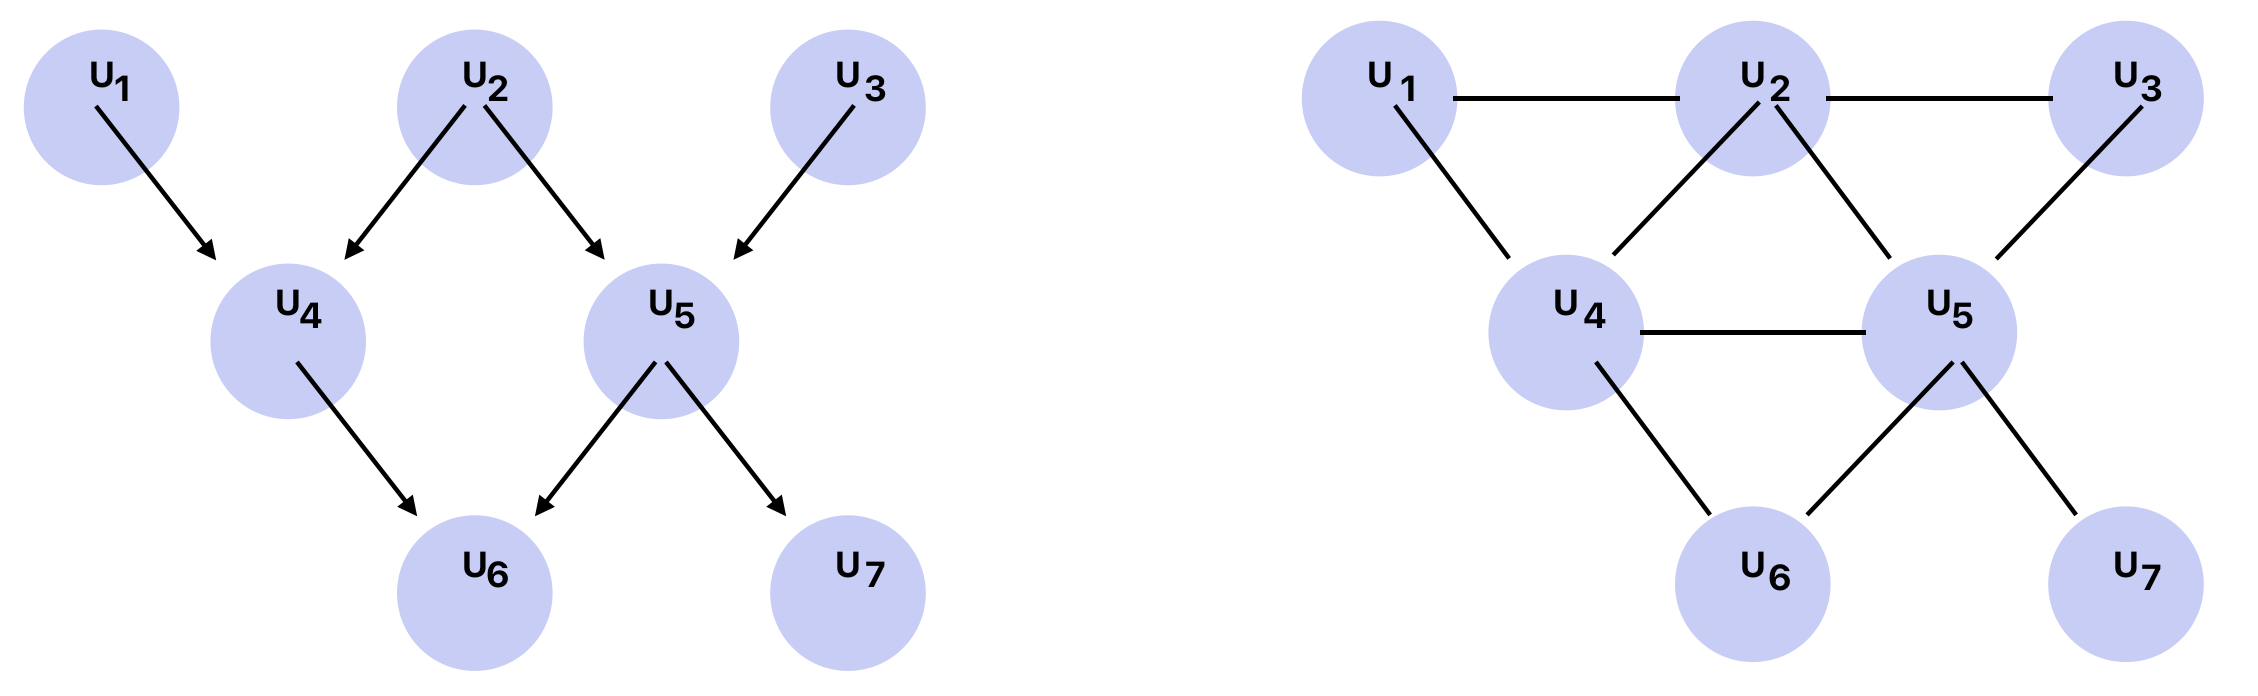
\includegraphics[width=1\linewidth]{Figures/GMRF Sparrows.png}
    \caption[Illustration of a pedigree as a GMRF]{Illustration of a pedigree as a GMRF, figure and figure text inspired by Figure 1 in \citet{Stensland_GMRF_bayes_animal_model}. On the left, a pedigree structure is depicted as a directed acyclic graph (DAG), where birds $U_1$ and $U_2$ are the parents of bird $U_4$, birds $U_2$ and $U_3$ the parents of bird $U_5$, and birds $U_4$ and $U_5$ the parents of bird $U_6$. Bird $U_7$ has one known parent in $U_5$, and one unknown. On the right, the conditional independence graph of the pedigree structure is given, where the parents sharing offspring is assigned an edge and the direction is removed.}
    \label{fig:GMRF_animal_model}
\end{figure}

% \subsection{Single and Multitrait Animal Model}
% When modelling the observed phenotypic trait values of individuals in a population, caution must be made when modelling the genetic component of the trait using INLA.
% If only one trait is considered, 
% The breeding values $\boldsymbol{\alpha}$ of an individual represents the genetic component of an observed phenotypic trait. 
% FINSIH THIS PART



% Would it be correct to interpret this as meaning that all the covariance is explained by relatedness, and that the additive variance is a scalar? Or is there a more complex covariance structure that might be present?
